% Examined Design — draft. Build: xelatex examined-design.tex (twice, for references).
% Decisions behind the text: decisions.md. Article plan: outline.md. Sources: research/*.md.
% Figures: figures/figs.tex (TikZ, pgfplots); board renders: figures/boards (figures/shoot.py, figures/crop.py).
\documentclass[11pt,a4paper]{article}

\usepackage{fontspec}
\setmainfont{Iowan Old Style}
\newfontfamily\greekfont{Palatino}
\newcommand{\gr}[1]{{\greekfont #1}}

\usepackage[a4paper,top=24mm,bottom=26mm,inner=25mm,outer=25mm]{geometry}
\usepackage{microtype}
\usepackage{xcolor}
\usepackage{enumitem}
\usepackage{multicol}
\usepackage{graphicx}
\usepackage{tikz}
\usepackage{pgfplots}
\usepackage[font=small,labelfont=sc,labelsep=period,skip=4pt]{caption}
\usepackage[hidelinks]{hyperref}
% Figures for Examined Design. Each \Fig... macro draws one figure body (no float).
\usetikzlibrary{positioning,arrows.meta,calc,shapes.misc,fit,backgrounds,decorations.pathreplacing}
\definecolor{accent}{HTML}{B4500E}
\definecolor{ok}{HTML}{2F7D4F}
\definecolor{bad}{HTML}{B3261E}
\definecolor{line}{gray}{0.35}
\definecolor{soft}{gray}{0.93}
\tikzset{
  every picture/.style={line width=0.6pt, >={Stealth[length=2.2mm]}},
  box/.style={draw=line, rounded corners=2pt, align=center, inner sep=4pt, font=\small},
  hot/.style={box, draw=accent, fill=accent!7},
  note/.style={font=\footnotesize, align=center, text=black!75},
  tiny/.style={font=\scriptsize, align=center, text=black!70},
  flow/.style={->, draw=line},
}

% ---- Prologue: two lines of testimony -------------------------------------------------
\newcommand{\FigTwoLines}{%
\begin{tikzpicture}
  \node[box, minimum width=26mm, minimum height=12mm] (m) {The model};
  \node[hot, minimum width=26mm, minimum height=12mm, right=40mm of m] (d) {You,\\the designer};
  \node[box, minimum width=26mm, minimum height=12mm, right=40mm of d] (u) {The user};
  \draw[flow, line width=1pt] (m) -- node[above, note]{tells you} node[below, tiny]{you are the hearer} (d);
  \draw[flow, line width=1pt] (d) -- node[above, note, align=center]{tells, through\\the product} node[below, tiny]{you are the speaker} (u);
  \node[note, above=3mm of d, text=accent] {tied \;·\; tested \;·\; signed};
  \node[tiny, below=12mm of d, text width=120mm] (f)
    {the same three failures on both lines: \textit{a claim that lost its source} \;·\; \textit{a dropped qualifier} \;·\; \textit{a pass read as proof}};
  \draw[line, densely dotted] ($(m.east)!0.5!(d.west)+(0,-6mm)$) -- ($(f.north)+(-16mm,0)$);
  \draw[line, densely dotted] ($(d.east)!0.5!(u.west)+(0,-6mm)$) -- ($(f.north)+(16mm,0)$);
\end{tikzpicture}}

% ---- Prologue: the article and the three conditions ------------------------------------
\newcommand{\FigArticleShape}{%
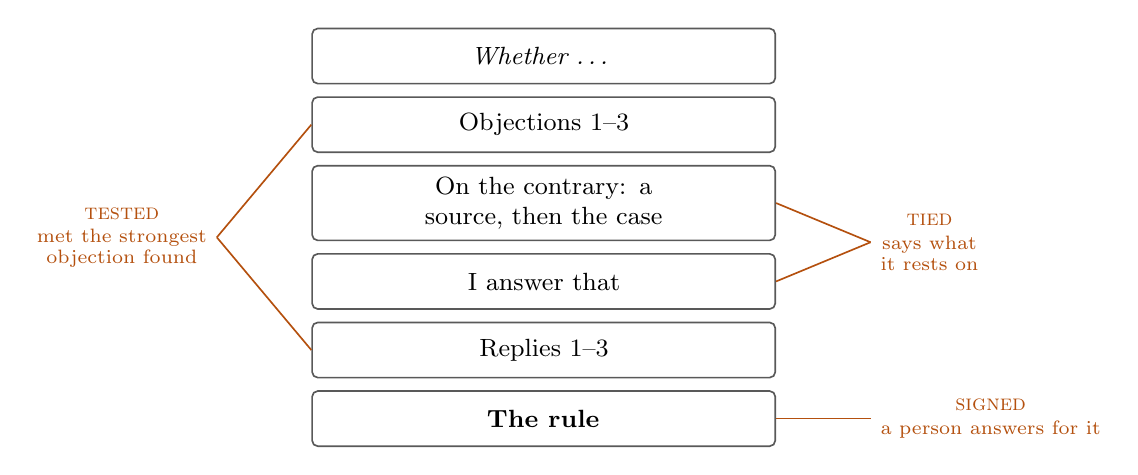
\begin{tikzpicture}[row/.style={box, text width=56mm, minimum height=7mm}]
  \node[row] (q) at (0,0) {\textit{Whether \dots}};
  \node[row, below=1.5mm of q] (o) {Objections 1--3};
  \node[row, below=1.5mm of o] (s) {On the contrary: a source, then the case};
  \node[row, below=1.5mm of s] (a) {I answer that};
  \node[row, below=1.5mm of a] (r) {Replies 1--3};
  \node[row, below=1.5mm of r, font=\small\bfseries] (b) {The rule};
  \node[note, text=accent, anchor=east] (te) at ($(o.west)!0.5!(r.west)+(-12mm,0)$) {\textsc{tested}\\[-1pt]\scriptsize met the strongest\\[-2pt]\scriptsize objection found};
  \draw[accent] (te.east) -- (o.west); \draw[accent] (te.east) -- (r.west);
  \node[note, text=accent, anchor=west] (ti) at ($(s.east)!0.5!(a.east)+(12mm,0)$) {\textsc{tied}\\[-1pt]\scriptsize says what\\[-2pt]\scriptsize it rests on};
  \draw[accent] (ti.west) -- (s.east); \draw[accent] (ti.west) -- (a.east);
  \node[note, text=accent, anchor=west] (si) at ($(b.east)+(12mm,0)$) {\textsc{signed}\\[-1pt]\scriptsize a person answers for it};
  \draw[accent] (si.west) -- (b.east);
\end{tikzpicture}}

% ---- The loop: going out and coming back -------------------------------------------------
\newcommand{\FigLoop}{%
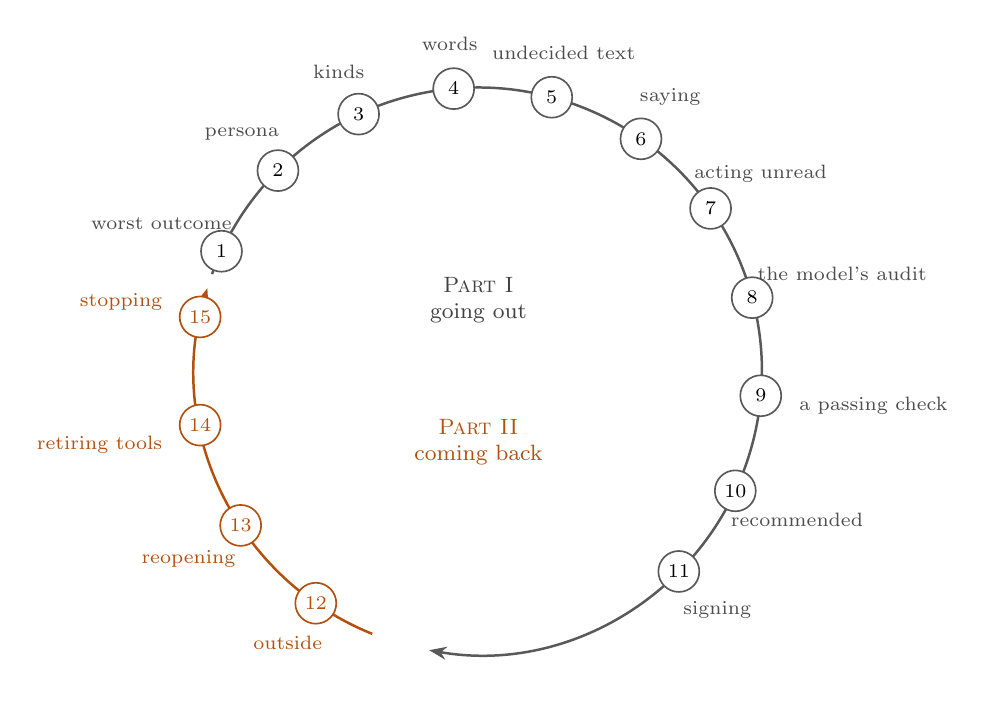
\begin{tikzpicture}
  \def\R{36mm}
  \draw[line, ->, line width=0.9pt] (160:\R) arc[start angle=160, end angle=-100, radius=\R];
  \draw[accent, ->, line width=0.9pt] (-112:\R) arc[start angle=-112, end angle=-197, radius=\R];
  \foreach \n/\a/\t in {1/155/worst outcome,2/135/persona,3/115/kinds,4/95/words,5/75/undecided text,6/55/saying,7/35/acting unread,8/15/the model's audit,9/-5/a passing check,10/-25/recommended,11/-45/signing}{
    \node[circle, draw=line, fill=white, inner sep=1.2pt, minimum size=5.2mm, font=\scriptsize] at (\a:\R) {\n};
    \node[tiny, anchor={\a+180}] at (\a:\R+3.6mm) {\t};
  }
  \foreach \n/\a/\t in {12/-125/outside,13/-147/reopening,14/-169/retiring tools,15/-191/stopping}{
    \node[circle, draw=accent, fill=white, inner sep=1.2pt, minimum size=5.2mm, font=\scriptsize, text=accent] at (\a:\R) {\n};
    \node[tiny, anchor={\a+180}, text=accent] at (\a:\R+3.6mm) {\t};
  }
  \node[note] at (0,9mm) {\textsc{Part I}\\going out};
  \node[note, text=accent] at (0,-9mm) {\textsc{Part II}\\coming back};
\end{tikzpicture}}

% ---- Article 1: what makes an outcome the worst ------------------------------------------
\newcommand{\FigWorst}{%
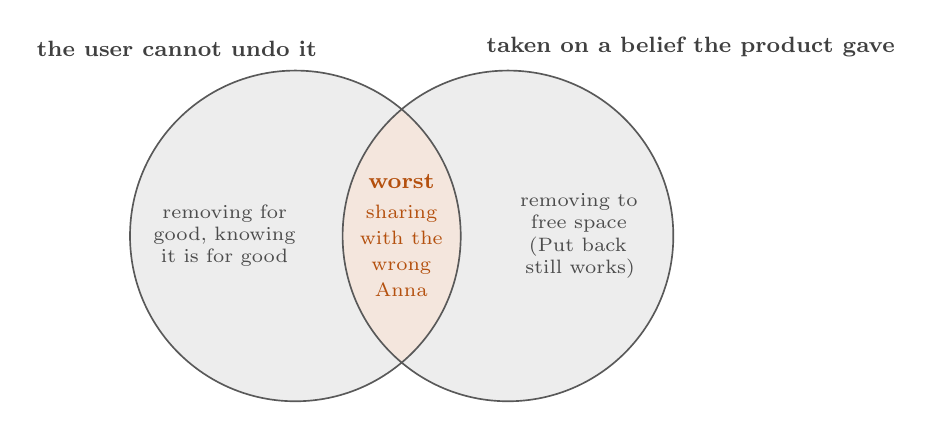
\begin{tikzpicture}
  \fill[soft] (0,0) circle (21mm);
  \fill[soft] (27mm,0) circle (21mm);
  \begin{scope}
    \clip (0,0) circle (21mm);
    \fill[accent!14] (27mm,0) circle (21mm);
  \end{scope}
  \draw[line] (0,0) circle (21mm) (27mm,0) circle (21mm);
  \node[note, font=\footnotesize\bfseries, anchor=south east] at (4mm,21.5mm) {the user cannot undo it};
  \node[note, font=\footnotesize\bfseries, anchor=south west] at (23mm,21.5mm) {taken on a belief the product gave};
  \node[tiny, text width=19mm] at (-9mm,0) {removing for good, knowing it is for good};
  \node[tiny, text width=19mm] at (36mm,0) {removing to free space (Put back still works)};
  \node[note, text width=13mm, text=accent] at (13.5mm,0) {\textbf{worst}\\[1pt]\scriptsize sharing with the wrong Anna};
\end{tikzpicture}}

% ---- Article 2: a yardstick, a check, and the remainder ----------------------------------
\newcommand{\FigYardstick}{%
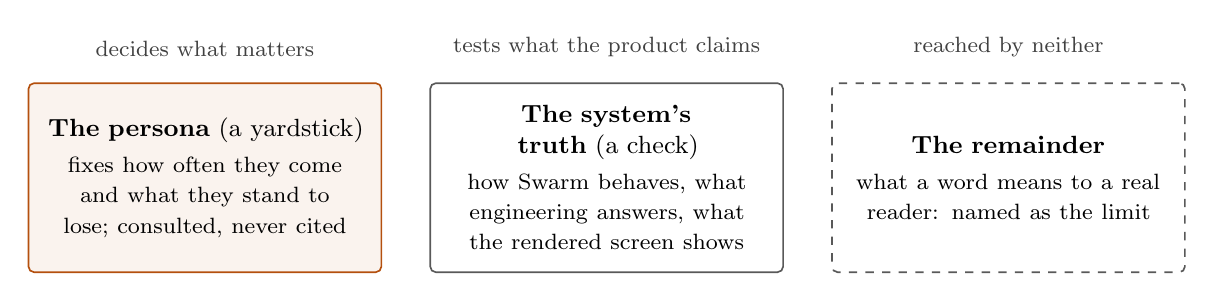
\begin{tikzpicture}
  \node[hot, text width=42mm, minimum height=24mm] (p) {\textbf{The persona} (a yardstick)\\[2pt]\footnotesize fixes how often they come and what they stand to lose; consulted, never cited};
  \node[box, text width=42mm, minimum height=24mm, right=6mm of p] (s) {\textbf{The system's truth} (a check)\\[2pt]\footnotesize how Swarm behaves, what engineering answers, what the rendered screen shows};
  \node[box, dashed, text width=42mm, minimum height=24mm, right=6mm of s] (r) {\textbf{The remainder}\\[2pt]\footnotesize what a word means to a real reader: named as the limit};
  \node[note, above=2mm of p] {decides what matters};
  \node[note, above=2mm of s] {tests what the product claims};
  \node[note, above=2mm of r] {reached by neither};
\end{tikzpicture}}

% ---- Article 3: a kind earns its place by an obligation ----------------------------------
\newcommand{\FigKinds}{%
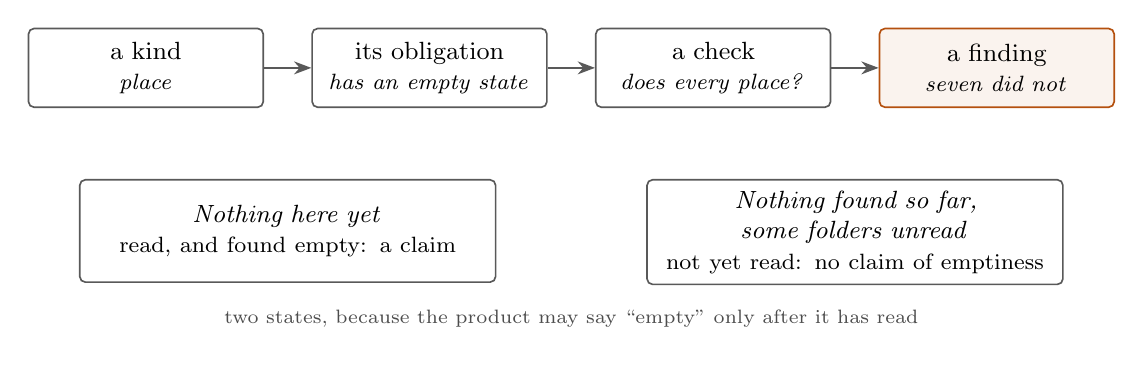
\begin{tikzpicture}[st/.style={box, minimum height=10mm, text width=27mm}]
  \node[st] (k) {a kind\\\footnotesize\textit{place}};
  \node[st, right=6mm of k] (o) {its obligation\\\footnotesize\textit{has an empty state}};
  \node[st, right=6mm of o] (c) {a check\\\footnotesize\textit{does every place?}};
  \node[hot, minimum height=10mm, text width=27mm, right=6mm of c] (f) {a finding\\\footnotesize\textit{seven did not}};
  \draw[flow] (k) -- (o); \draw[flow] (o) -- (c); \draw[flow] (c) -- (f);
  \node[box, text width=50mm, minimum height=13mm, anchor=north] (e) at ($(k.south)!0.5!(o.south)+(0,-9mm)$) {\textit{Nothing here yet}\\\footnotesize read, and found empty: a claim};
  \node[box, text width=50mm, minimum height=13mm, anchor=north] (n) at ($(c.south)!0.5!(f.south)+(0,-9mm)$) {\textit{Nothing found so far, some folders unread}\\\footnotesize not yet read: no claim of emptiness};
  \node[tiny, anchor=north] at ($(e.south)!0.5!(n.south)+(0,-2mm)$) {two states, because the product may say ``empty'' only after it has read};
\end{tikzpicture}}

% ---- Article 4: the implicature check ------------------------------------------------------
\newcommand{\FigImplicature}{%
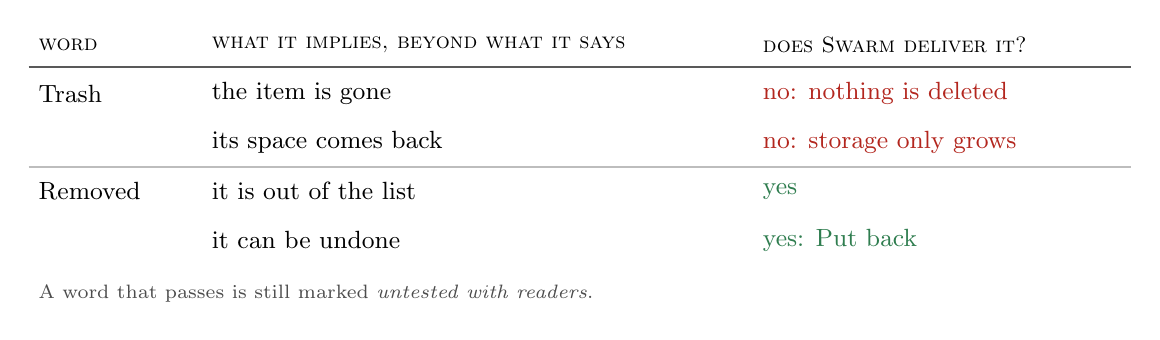
\begin{tikzpicture}[c/.style={font=\small, anchor=west}, y=6.2mm]
  \node[c, font=\footnotesize\scshape] at (0,0) {word};
  \node[c, font=\footnotesize\scshape] at (22mm,0) {what it implies, beyond what it says};
  \node[c, font=\footnotesize\scshape] at (92mm,0) {does Swarm deliver it?};
  \draw[line] (0,-0.45) -- (140mm,-0.45);
  \node[c] at (0,-1) {Trash}; \node[c] at (22mm,-1) {the item is gone}; \node[c, text=bad] at (92mm,-1) {no: nothing is deleted};
  \node[c] at (22mm,-2) {its space comes back}; \node[c, text=bad] at (92mm,-2) {no: storage only grows};
  \draw[line!40] (0,-2.5) -- (140mm,-2.5);
  \node[c] at (0,-3) {Removed}; \node[c] at (22mm,-3) {it is out of the list}; \node[c, text=ok] at (92mm,-3) {yes};
  \node[c] at (22mm,-4) {it can be undone}; \node[c, text=ok] at (92mm,-4) {yes: Put back};
  \node[tiny, anchor=west] at (0,-5.1) {A word that passes is still marked \textit{untested with readers}.};
\end{tikzpicture}}

% ---- Article 5: where undecided text may go -----------------------------------------------
\newcommand{\FigTextPath}{%
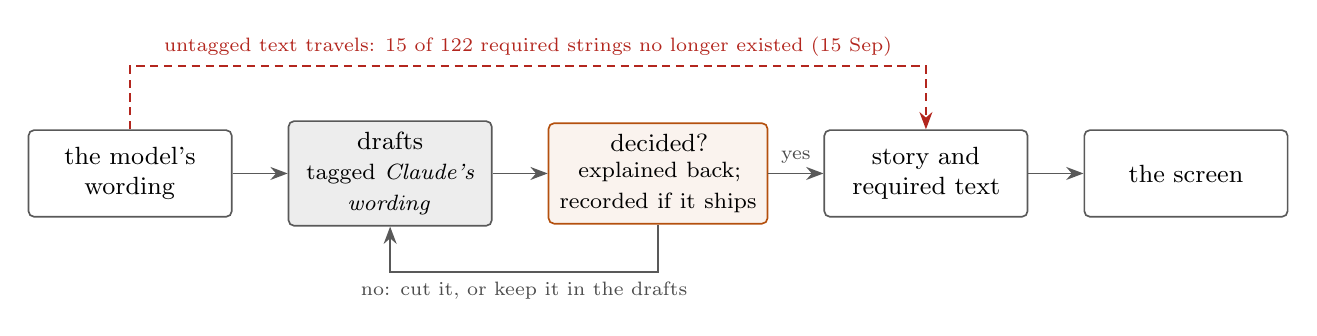
\begin{tikzpicture}[st/.style={box, minimum height=11mm, text width=23mm}]
  \node[st] (m) {the model's\\wording};
  \node[st, right=7mm of m, fill=soft] (d) {drafts\\\footnotesize tagged \textit{Claude's wording}};
  \node[hot, minimum height=11mm, text width=25mm, right=7mm of d] (g) {decided?\\\footnotesize explained back;\\recorded if it ships};
  \node[st, right=7mm of g] (s) {story and\\required text};
  \node[st, right=7mm of s] (u) {the screen};
  \draw[flow] (m) -- (d); \draw[flow] (d) -- (g); \draw[flow] (g) -- node[above, tiny]{yes} (s); \draw[flow] (s) -- (u);
  \draw[flow] (g.south) -- ++(0,-6mm) -| node[pos=0.25, below, tiny]{no: cut it, or keep it in the drafts} (d.south);
  \draw[->, bad, densely dashed] (m.north) -- ++(0,8mm) -| node[pos=0.25, above, tiny, text=bad]{untagged text travels: 15 of 122 required strings no longer existed (15 Sep)} (s.north);
\end{tikzpicture}}

% ---- Article 6: what was observed, and how far it reaches ----------------------------------
\newcommand{\FigObserved}{%
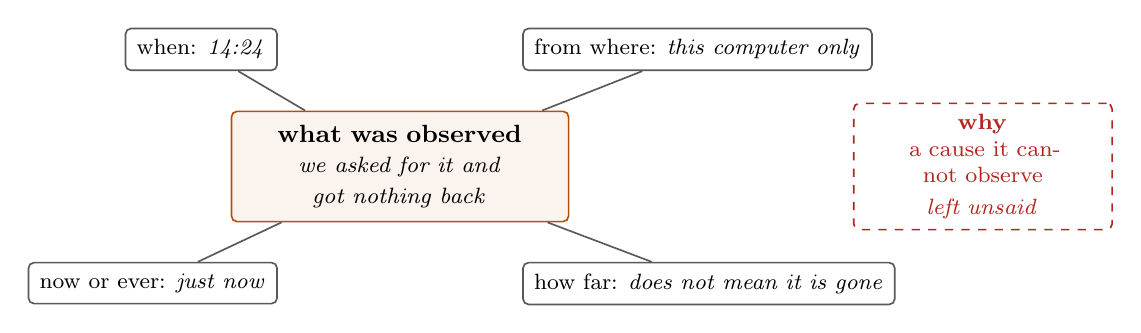
\begin{tikzpicture}
  \node[hot, text width=40mm, minimum height=14mm] (o) {\textbf{what was observed}\\\footnotesize\textit{we asked for it and got nothing back}};
  \node[box, above left=5mm and -6mm of o, font=\footnotesize] (w) {when: \textit{14:24}};
  \node[box, above right=5mm and -6mm of o, font=\footnotesize] (f) {from where: \textit{this computer only}};
  \node[box, below left=5mm and -6mm of o, font=\footnotesize] (n) {now or ever: \textit{just now}};
  \node[box, below right=5mm and -6mm of o, font=\footnotesize] (h) {how far: \textit{does not mean it is gone}};
  \foreach \x in {w,f,n,h} \draw[line] (o) -- (\x);
  \node[box, dashed, draw=bad, right=36mm of o, text width=30mm, font=\footnotesize, text=bad] (y) {\textbf{why}\\a cause it cannot observe\\[2pt]\textit{left unsaid}};
\end{tikzpicture}}

% ---- Article 7: the life of a read ---------------------------------------------------------
\newcommand{\FigRead}{%
\begin{tikzpicture}[seg/.style={box, minimum height=17mm, font=\footnotesize, text width=##1}, x=1mm]
  \node[seg=19mm, fill=white] (a) at (0,0) {a short pause\\\textit{nothing shown}};
  \node[seg=27mm, fill=soft, right=0mm of a] (b) {placeholders\\\textit{``Reading your list\dots''}};
  \node[seg=27mm, fill=soft, right=0mm of b] (c) {if it runs long\\\textit{``taking longer than usual''}};
  \node[box, draw=ok, minimum height=8mm, text width=40mm, font=\footnotesize, right=7mm of c, yshift=7mm] (r) {read: figures and badges shown};
  \node[box, draw=bad, minimum height=8mm, text width=40mm, font=\footnotesize, right=7mm of c, yshift=-7mm] (x) {failed: last read kept, \textit{with its time}; Try again};
  \draw[flow] (c.east) -- (r.west); \draw[flow] (c.east) -- (x.west);
  \draw[line, ->] ($(a.north west)+(0,4mm)$) -- node[above, tiny, pos=0.5]{time} ($(c.north east)+(0,4mm)$);
  \node[font=\footnotesize, anchor=east] at ($(a.south west)+(-2mm,-6mm)$) {commit};
  \draw[bad, line width=2pt] ($(a.south west)+(0,-6mm)$) -- ($(c.south east)+(0,-6mm)$);
  \node[tiny, text=bad, anchor=north] at ($(b.south)!0.5!(c.south)+(0,-7mm)$) {off until its facts are read};
  \node[font=\footnotesize, anchor=east] at ($(a.south west)+(-2mm,-13mm)$) {cancel};
  \draw[ok, line width=2pt] ($(a.south west)+(0,-13mm)$) -- ($(x.east |- a.south)+(0,-13mm)$);
  \node[tiny, text=ok, anchor=north] at ($(b.south)!0.5!(c.south)+(0,-14mm)$) {always works};
  \node[tiny, text=ok, anchor=west] at ($(r.east)+(1mm,0)$) {commit on};
  \node[tiny, text=bad, anchor=west] at ($(x.east)+(1mm,0)$) {commit off};
\end{tikzpicture}}

% ---- Charts redrawn from studies (numbers exactly as in research/*.md) --------------------
\pgfplotsset{compat=1.18,
  every axis/.append style={font=\scriptsize, axis line style={line}, tick style={line}, label style={font=\footnotesize}},
}

% Article 3: Nielsen (1994), cumulative variance explained by factors (text of the paper).
\newcommand{\ChartNielsen}{%
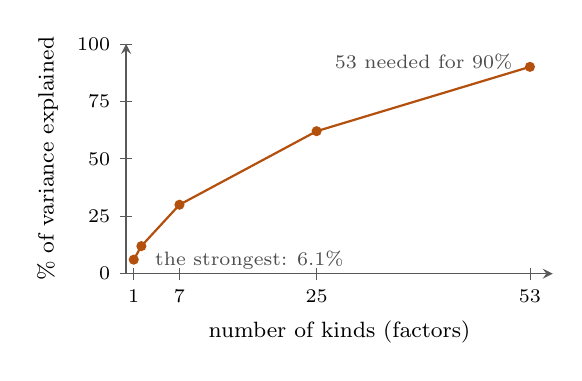
\begin{tikzpicture}
\begin{axis}[width=70mm, height=45mm, xmin=0, xmax=56, ymin=0, ymax=100,
  xlabel={number of kinds (factors)}, ylabel={\% of variance explained},
  xtick={1,7,25,53}, ytick={0,25,50,75,100}, axis lines=left, clip=false]
  \addplot[accent, mark=*, mark size=1.4pt, line width=0.8pt] coordinates {(1,6.1) (2,12.0) (7,30) (25,62) (53,90)};
  \node[tiny, anchor=west] at (axis cs:2.5,6) {the strongest: 6.1\%};
  \node[tiny, anchor=east] at (axis cs:52,92) {53 needed for 90\%};
\end{axis}
\end{tikzpicture}}

% Article 4: Doshi & Hauser (2024), Figs 2 and 4; effects of one / five AI ideas.
\newcommand{\ChartDoshi}{%
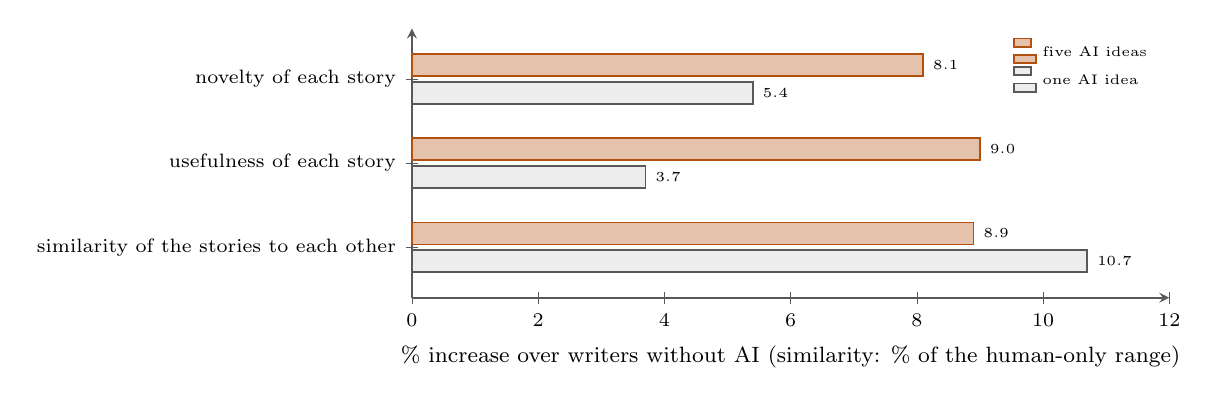
\begin{tikzpicture}
\begin{axis}[width=112mm, height=50mm, xbar, bar width=2.8mm, xmin=0, xmax=12, clip=false,
  ymin=-0.6, ymax=2.6, ytick={0,1,2}, yticklabels={similarity of the stories to each other,usefulness of each story,novelty of each story}, xlabel={\% increase over writers without AI (similarity: \% of the human-only range)}, axis lines=left,
  nodes near coords, every node near coord/.append style={font=\tiny, /pgf/number format/fixed, /pgf/number format/precision=1, /pgf/number format/fixed zerofill},
  legend style={font=\tiny, draw=none, at={(0.99,0.99)}, anchor=north east}, legend cell align=left, reverse legend]
  \addplot[fill=soft, draw=line] coordinates {(10.7,0) (3.7,1) (5.4,2)};
  \addplot[fill=accent!35, draw=accent] coordinates {(8.9,0) (9.0,1) (8.1,2)};
  \legend{one AI idea, five AI ideas}
\end{axis}
\end{tikzpicture}}

% Article 6: van der Bles et al. (2020), Fig. 5, internal meta-analysis of experiments 1-4 (Cohen's d).
\newcommand{\ChartVanDerBles}{%
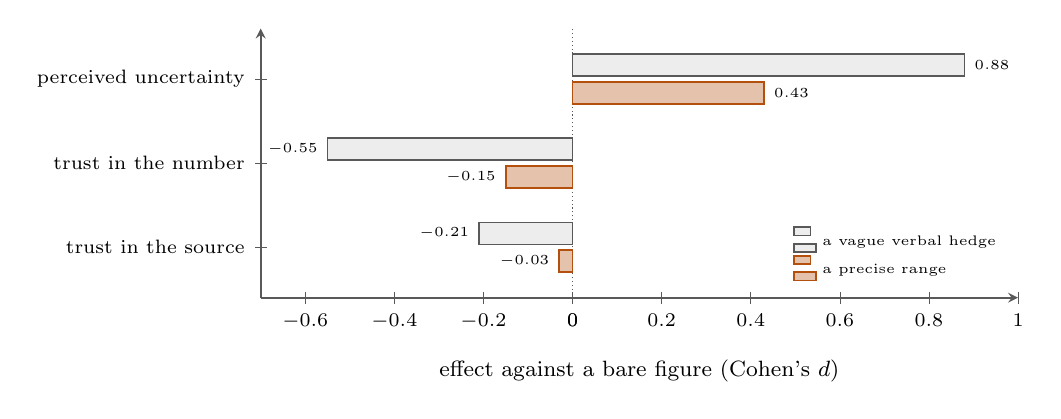
\begin{tikzpicture}
\begin{axis}[width=112mm, height=50mm, xbar, bar width=2.8mm, xmin=-0.7, xmax=1.0, clip=false,
  ymin=-0.6, ymax=2.6, ytick={0,1,2}, yticklabels={trust in the source,trust in the number,perceived uncertainty}, xlabel={effect against a bare figure (Cohen's $d$)}, axis lines=left,
  extra x ticks={0}, extra x tick style={grid=major, grid style={line, densely dotted}},
  nodes near coords, every node near coord/.append style={font=\tiny, /pgf/number format/fixed, /pgf/number format/precision=2, /pgf/number format/fixed zerofill},
  legend style={font=\tiny, draw=none, at={(0.99,0.03)}, anchor=south east}, legend cell align=left, reverse legend]
  \addplot[fill=accent!35, draw=accent] coordinates {(-0.03,0) (-0.15,1) (0.43,2)};
  \addplot[fill=soft, draw=line] coordinates {(-0.21,0) (-0.55,1) (0.88,2)};
  \legend{a precise range, a vague verbal hedge}
\end{axis}
\end{tikzpicture}}

% ---- Article 8: slices, a merge, and what the circle threatens ------------------------------
\newcommand{\FigAudit}{%
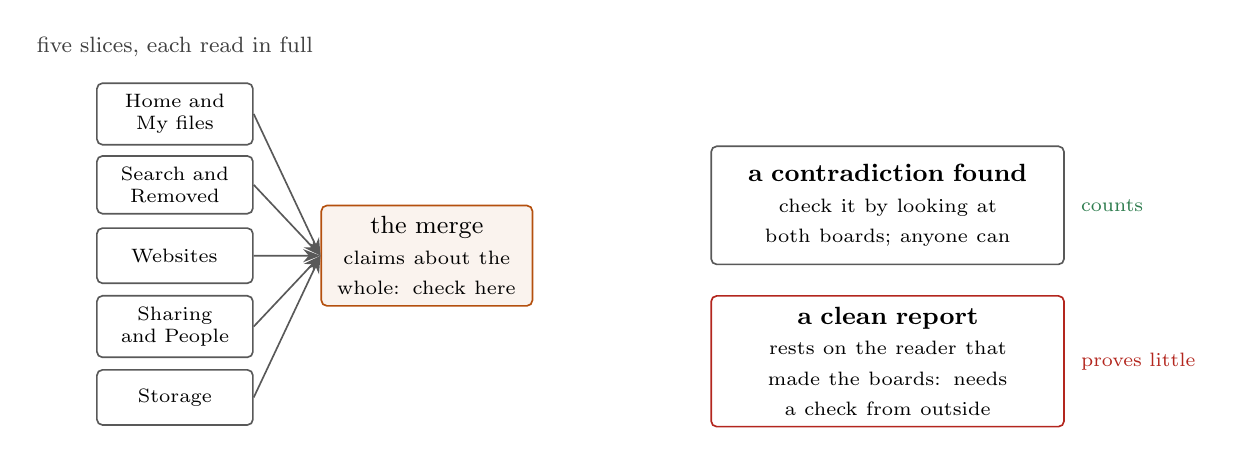
\begin{tikzpicture}[sl/.style={box, minimum width=17mm, minimum height=7mm, font=\scriptsize}]
  \foreach \i/\t in {0/Home and My files,1/Search and Removed,2/Websites,3/Sharing and People,4/Storage}{
    \node[sl, text width=17mm] (s\i) at (0,-\i*9mm) {\t};
  }
  \node[hot, text width=24mm, minimum height=12mm] (mg) at (32mm,-18mm) {the merge\\\scriptsize claims about the whole: check here};
  \foreach \i in {0,...,4} \draw[flow] (s\i.east) -- (mg.west);
  \node[note, above=2mm of s0] {five slices, each read in full};
  \begin{scope}[xshift=68mm, yshift=-4mm]
    \node[box, text width=42mm, minimum height=15mm, anchor=north west] (f) at (0,0) {\textbf{a contradiction found}\\\scriptsize check it by looking at both boards; anyone can};
    \node[box, draw=bad, text width=42mm, minimum height=15mm, anchor=north west] (c) at (0,-19mm) {\textbf{a clean report}\\\scriptsize rests on the reader that made the boards: needs a check from outside};
    \node[tiny, text=ok, anchor=west] at (f.east) {\;counts};
    \node[tiny, text=bad, anchor=west] at (c.east) {\;proves little};
  \end{scope}
\end{tikzpicture}}

% Article 8: Liu et al. (2024), arXiv v3 Table 6; gpt-3.5-turbo-0613, 20 documents.
\newcommand{\ChartLiu}{%
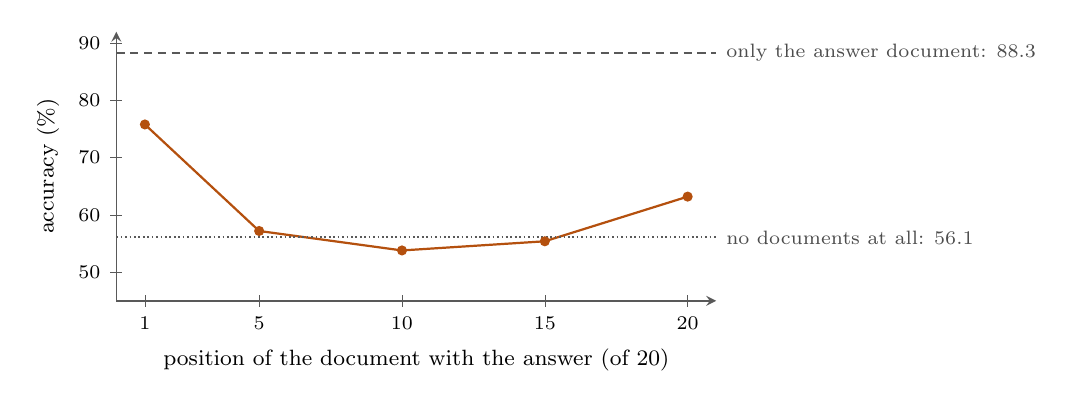
\begin{tikzpicture}
\begin{axis}[width=92mm, height=50mm, xmin=0, xmax=21, ymin=45, ymax=92, axis lines=left,
  xtick={1,5,10,15,20}, ytick={50,60,70,80,90}, xlabel={position of the document with the answer (of 20)}, ylabel={accuracy (\%)}, clip=false]
  \addplot[accent, mark=*, mark size=1.4pt, line width=0.8pt] coordinates {(1,75.8) (5,57.2) (10,53.8) (15,55.4) (20,63.2)};
  \draw[line, densely dashed] (axis cs:0,88.3) -- (axis cs:21,88.3) node[tiny, anchor=west]{only the answer document: 88.3};
  \draw[line, densely dotted] (axis cs:0,56.1) -- (axis cs:21,56.1) node[tiny, anchor=west]{no documents at all: 56.1};
\end{axis}
\end{tikzpicture}}

% ---- Article 9: the veil (project data) and what each check cannot see -----------------------
\newcommand{\ChartVeil}{%
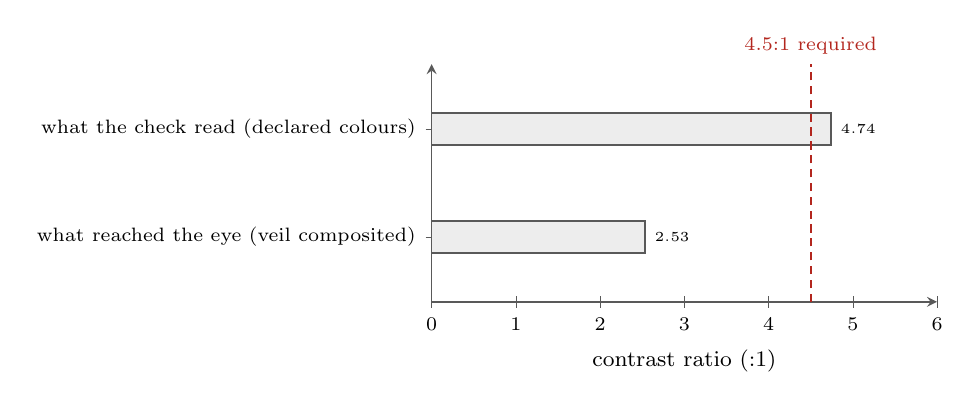
\begin{tikzpicture}
\begin{axis}[width=80mm, height=46mm, xbar, bar width=4mm, xmin=0, xmax=6, clip=false,
  ymin=-0.6, ymax=1.6, ytick={0,1}, yticklabels={what reached the eye (veil composited),what the check read (declared colours)},
  xlabel={contrast ratio (:1)}, axis lines=left, nodes near coords, every node near coord/.append style={font=\tiny, /pgf/number format/fixed, /pgf/number format/precision=2, /pgf/number format/fixed zerofill}]
  \addplot[fill=soft, draw=line] coordinates {(2.53,0) (4.74,1)};
  \draw[bad, densely dashed] (axis cs:4.5,-0.6) -- (axis cs:4.5,1.6) node[tiny, text=bad, anchor=south]{4.5:1 required};
\end{axis}
\end{tikzpicture}}

\newcommand{\FigCannotSee}{%
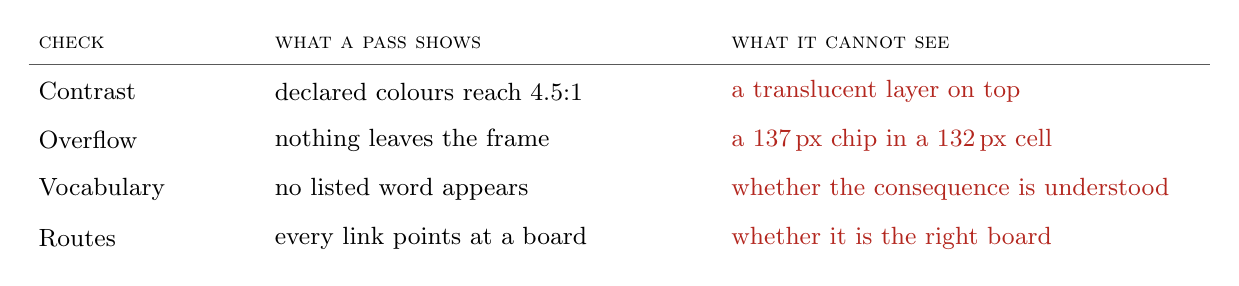
\begin{tikzpicture}[c/.style={font=\small, anchor=west}, y=6.2mm]
  \node[c, font=\footnotesize\scshape] at (0,0) {check}; \node[c, font=\footnotesize\scshape] at (30mm,0) {what a pass shows}; \node[c, font=\footnotesize\scshape] at (88mm,0) {what it cannot see};
  \draw[line] (0,-0.45) -- (150mm,-0.45);
  \node[c] at (0,-1) {Contrast}; \node[c] at (30mm,-1) {declared colours reach 4.5:1}; \node[c, text=bad] at (88mm,-1) {a translucent layer on top};
  \node[c] at (0,-2) {Overflow}; \node[c] at (30mm,-2) {nothing leaves the frame}; \node[c, text=bad] at (88mm,-2) {a 137\,px chip in a 132\,px cell};
  \node[c] at (0,-3) {Vocabulary}; \node[c] at (30mm,-3) {no listed word appears}; \node[c, text=bad] at (88mm,-3) {whether the consequence is understood};
  \node[c] at (0,-4) {Routes}; \node[c] at (30mm,-4) {every link points at a board}; \node[c, text=bad] at (88mm,-4) {whether it is the right board};
\end{tikzpicture}}

% ---- Article 10: defaults (Johnson & Goldstein 2003, online experiment) and this paper's record --
\newcommand{\ChartDefaults}{%
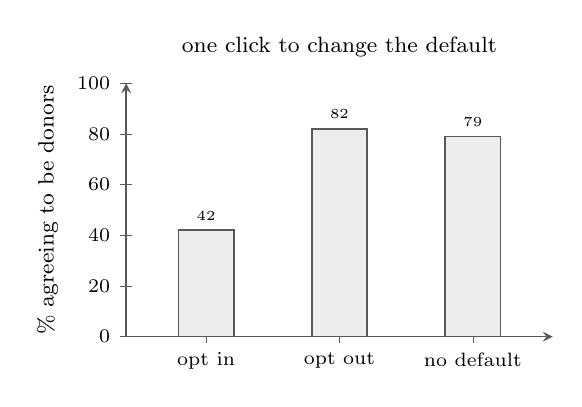
\begin{tikzpicture}
\begin{axis}[width=70mm, height=48mm, ybar, bar width=7mm, ymin=0, ymax=100, axis lines=left,
  xmin=0.4, xmax=3.6, xtick={1,2,3}, xticklabels={opt in,opt out,no default}, ylabel={\% agreeing to be donors},
  title={\footnotesize one click to change the default}, nodes near coords, every node near coord/.append style={font=\tiny}]
  \addplot[fill=soft, draw=line] coordinates {(1,42) (2,82) (3,79)};
\end{axis}
\end{tikzpicture}\hspace{6mm}%
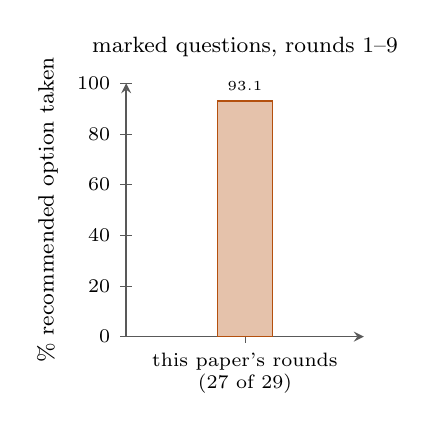
\begin{tikzpicture}
\begin{axis}[width=46mm, height=48mm, ybar, bar width=7mm, ymin=0, ymax=100, axis lines=left,
  xmin=0.4, xmax=1.6, xtick={1}, xticklabels={this paper's rounds\\(27 of 29)}, xticklabel style={align=center}, ylabel={\% recommended option taken},
  title={\footnotesize marked questions, rounds 1--9}, nodes near coords, every node near coord/.append style={font=\tiny}]
  \addplot[fill=accent!35, draw=accent] coordinates {(1,93.1)};
\end{axis}
\end{tikzpicture}}

\newcommand{\FigEcho}{%
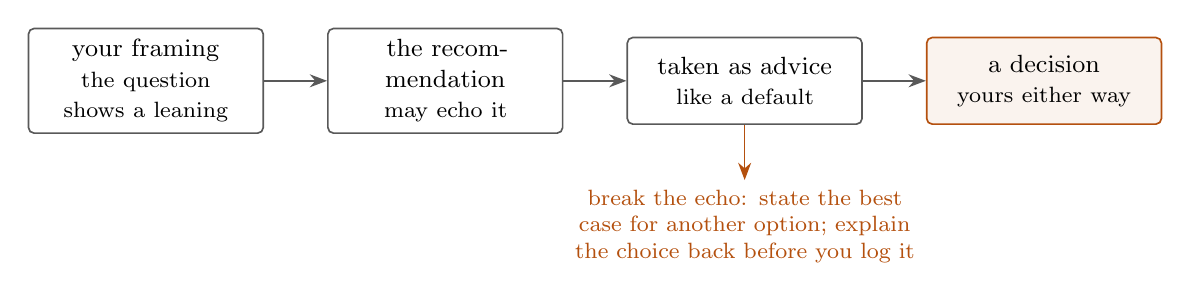
\begin{tikzpicture}[st/.style={box, minimum height=11mm, text width=27mm}]
  \node[st] (y) {your framing\\\footnotesize the question shows a leaning};
  \node[st, right=8mm of y] (m) {the recommendation\\\footnotesize may echo it};
  \node[st, right=8mm of m] (t) {taken as advice\\\footnotesize like a default};
  \node[hot, minimum height=11mm, text width=27mm, right=8mm of t] (d) {a decision\\\footnotesize yours either way};
  \draw[flow] (y) -- (m); \draw[flow] (m) -- (t); \draw[flow] (t) -- (d);
  \draw[->, accent] (t.south) -- ++(0,-7mm) node[below, note, text=accent, text width=60mm] {break the echo: state the best case for another option; explain the choice back before you log it};
\end{tikzpicture}}

% ---- Article 11: the chain from a screen to a signature ---------------------------------------
\newcommand{\FigSignChain}{%
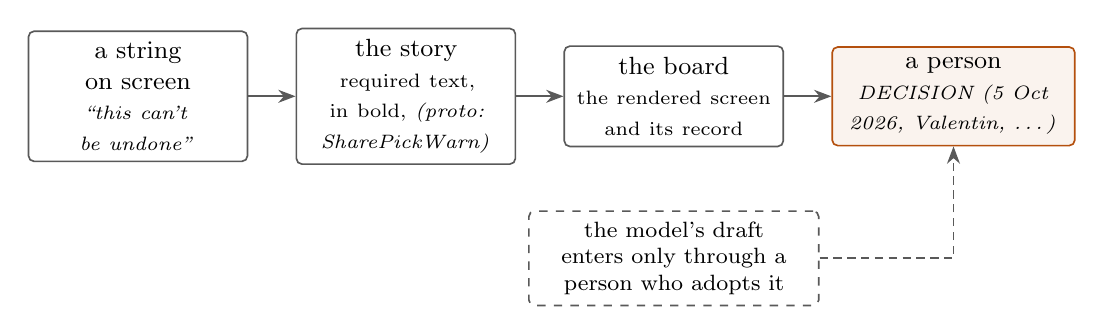
\begin{tikzpicture}[st/.style={box, minimum height=12mm, text width=25mm}]
  \node[st] (s) {a string on screen\\\scriptsize\textit{``this can't be undone''}};
  \node[st, right=6mm of s] (j) {the story\\\scriptsize required text, in bold, \textit{(proto: SharePickWarn)}};
  \node[st, right=6mm of j] (b) {the board\\\scriptsize the rendered screen and its record};
  \node[hot, minimum height=12mm, text width=28mm, right=6mm of b] (p) {a person\\\scriptsize\textit{DECISION (5 Oct 2026, Valentin, \dots)}};
  \draw[flow] (s) -- (j); \draw[flow] (j) -- (b); \draw[flow] (b) -- (p);
  \node[box, dashed, text width=34mm, font=\footnotesize, below=8mm of b] (m) {the model's draft enters only through a person who adopts it};
  \draw[flow, densely dashed] (m.east) -| (p.south);
\end{tikzpicture}}

% ---- Article 12: the circle and what lies outside it -----------------------------------------
\newcommand{\FigOutside}{%
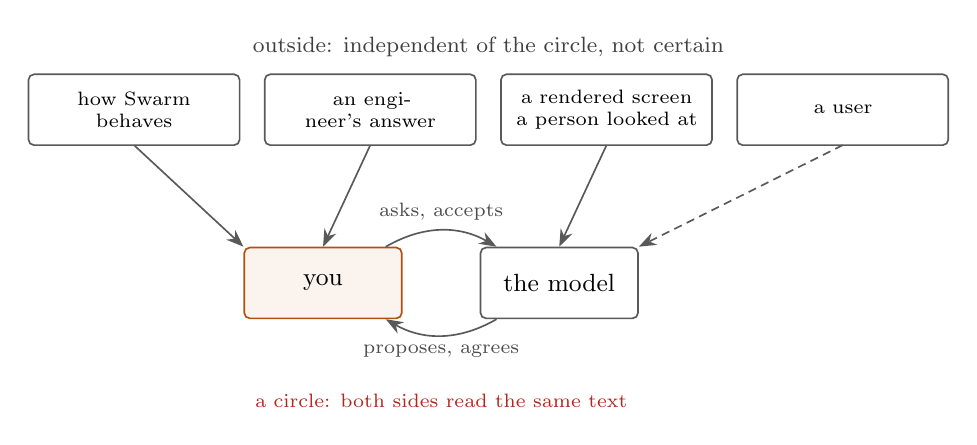
\begin{tikzpicture}
  \node[hot, minimum width=20mm, minimum height=9mm] (d) at (0,0) {you};
  \node[box, minimum width=20mm, minimum height=9mm] (m) at (30mm,0) {the model};
  \draw[flow, bend left=30] (d) to node[above, tiny]{asks, accepts} (m);
  \draw[flow, bend left=30] (m) to node[below, tiny]{proposes, agrees} (d);
  \node[tiny, text=bad] at (15mm,-15mm) {a circle: both sides read the same text};
  \foreach \t/\x in {how Swarm behaves/-24,an engineer's answer/6,a rendered screen a person looked at/36,a user/66}{
    \node[box, font=\scriptsize, text width=24mm, minimum height=9mm] (o) at (\x mm,22mm) {\t};
  }
  \draw[flow] (-24mm,17.5mm) -- (d.north west);
  \draw[flow] (6mm,17.5mm) -- (d.north);
  \draw[flow] (36mm,17.5mm) -- (m.north);
  \draw[flow, densely dashed] (66mm,17.5mm) -- (m.north east);
  \node[note] at (21mm,30mm) {outside: independent of the circle, not certain};
\end{tikzpicture}}

% Article 12: Huang et al. (2024), Tables 2-3, GPT-3.5.
\newcommand{\ChartHuang}{%
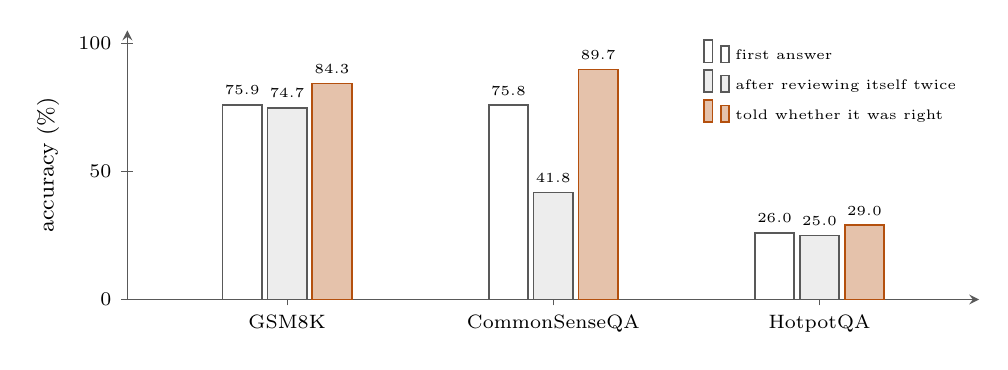
\begin{tikzpicture}
\begin{axis}[width=124mm, height=50mm, ybar=2pt, bar width=5mm, ymin=0, ymax=105, axis lines=left,
  xmin=0.4, xmax=3.6, xtick={1,2,3}, xticklabels={GSM8K,CommonSenseQA,HotpotQA}, ylabel={accuracy (\%)},
  nodes near coords, every node near coord/.append style={font=\tiny, /pgf/number format/fixed, /pgf/number format/precision=1, /pgf/number format/fixed zerofill},
  legend style={font=\tiny, draw=none, at={(0.99,0.99)}, anchor=north east}, legend cell align=left]
  \addplot[fill=white, draw=line] coordinates {(1,75.9) (2,75.8) (3,26.0)};
  \addplot[fill=soft, draw=line] coordinates {(1,74.7) (2,41.8) (3,25.0)};
  \addplot[fill=accent!35, draw=accent] coordinates {(1,84.3) (2,89.7) (3,29.0)};
  \legend{first answer, after reviewing itself twice, told whether it was right}
\end{axis}
\end{tikzpicture}}

% ---- Article 13: when to reopen -----------------------------------------------------------------
\newcommand{\FigReopen}{%
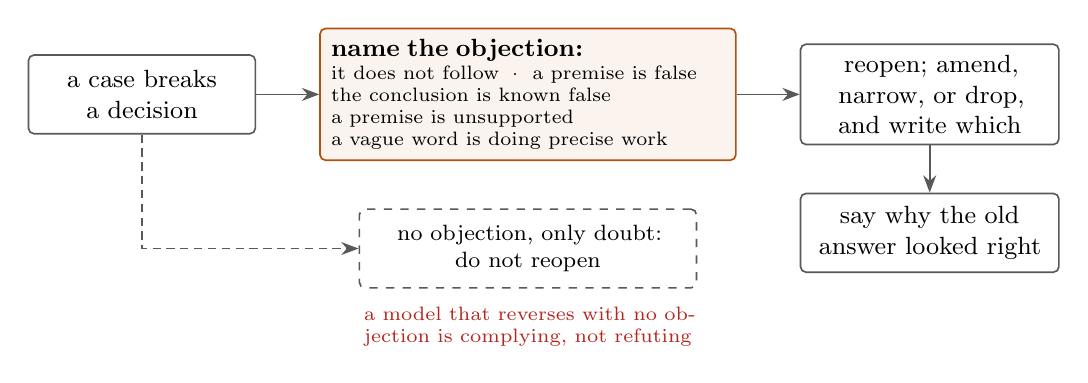
\begin{tikzpicture}[st/.style={box, minimum height=10mm}]
  \node[st, text width=26mm] (c) {a case breaks a decision};
  \node[hot, text width=50mm, right=8mm of c, align=left, font=\scriptsize] (o) {\textbf{\small name the objection:}\\
    it does not follow \;·\; a premise is false\\the conclusion is known false\\a premise is unsupported\\a vague word is doing precise work};
  \node[st, text width=30mm, right=8mm of o] (r) {reopen; amend, narrow, or drop, and write which};
  \node[st, text width=30mm, below=6mm of r] (e) {say why the old answer looked right};
  \draw[flow] (c) -- (o); \draw[flow] (o) -- (r); \draw[flow] (r) -- (e);
  \node[st, dashed, text width=40mm, below=6mm of o, font=\footnotesize] (n) {no objection, only doubt: \\do not reopen};
  \draw[flow, densely dashed] (c.south) |- (n.west);
  \node[tiny, text=bad, below=1mm of n, text width=50mm] {a model that reverses with no objection is complying, not refuting};
\end{tikzpicture}}

% Article 13: Wang, Yue & Sun (2023), Table 2; ChatGPT, share of correct answers abandoned under invalid argument.
\newcommand{\ChartWang}{%
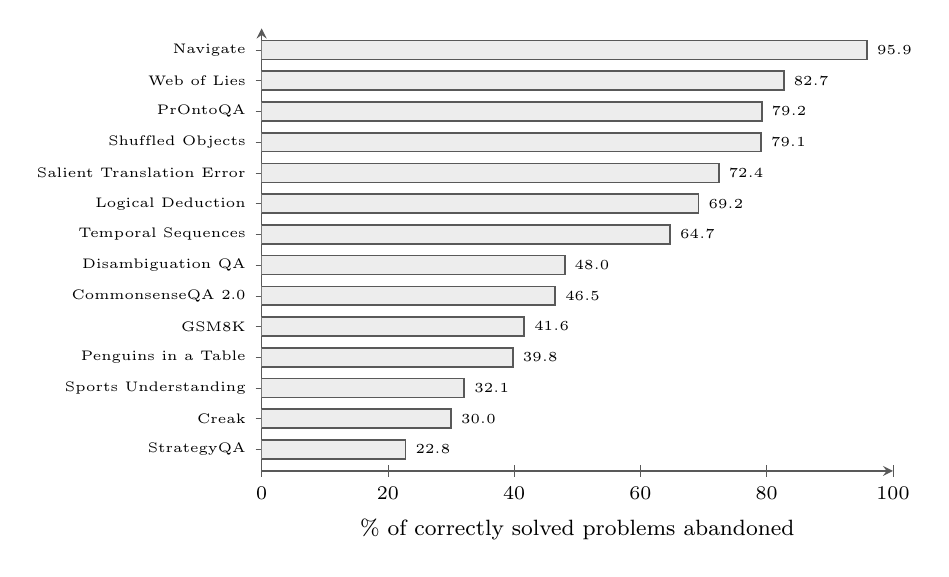
\begin{tikzpicture}
\begin{axis}[width=96mm, height=72mm, xbar, bar width=2.4mm, xmin=0, xmax=100, axis lines=left,
  ymin=0.3, ymax=14.7, ytick={1,...,14}, yticklabels={StrategyQA,Creak,Sports Understanding,Penguins in a Table,GSM8K,CommonsenseQA 2.0,Disambiguation QA,Temporal Sequences,Logical Deduction,Salient Translation Error,Shuffled Objects,PrOntoQA,Web of Lies,Navigate},
  y tick label style={font=\tiny}, xlabel={\% of correctly solved problems abandoned}, nodes near coords, every node near coord/.append style={font=\tiny, /pgf/number format/fixed, /pgf/number format/precision=1, /pgf/number format/fixed zerofill}]
  \addplot[fill=soft, draw=line] coordinates {(22.8,1) (30.0,2) (32.1,3) (39.8,4) (41.6,5) (46.5,6) (48.0,7) (64.7,8) (69.2,9) (72.4,10) (79.1,11) (79.2,12) (82.7,13) (95.9,14)};
\end{axis}
\end{tikzpicture}}

% ---- Article 14: tools and claims ------------------------------------------------------------
\newcommand{\FigToolsClaims}{%
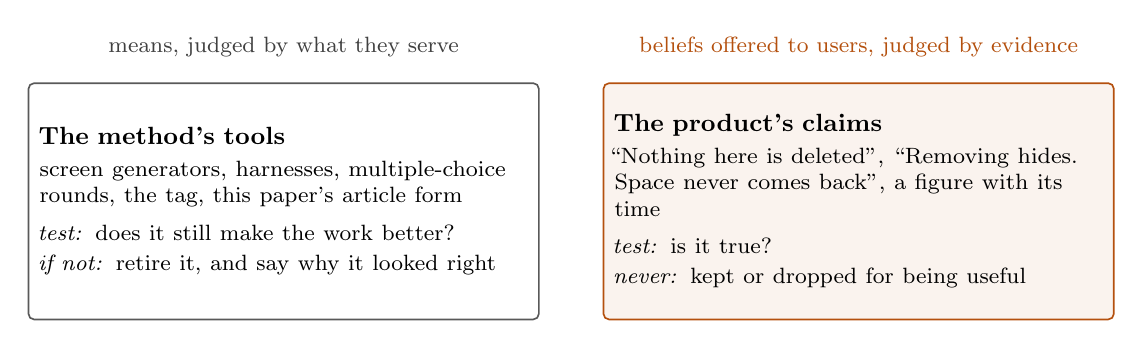
\begin{tikzpicture}
  \node[box, text width=62mm, minimum height=30mm, align=left] (t) {\textbf{The method's tools}\\[2pt]\footnotesize screen generators, harnesses, multiple-choice rounds, the tag, this paper's article form\\[4pt]\textit{test:} does it still make the work better?\\\textit{if not:} retire it, and say why it looked right};
  \node[hot, text width=62mm, minimum height=30mm, align=left, right=8mm of t] (c) {\textbf{The product's claims}\\[2pt]\footnotesize ``Nothing here is deleted'', ``Removing hides. Space never comes back'', a figure with its time\\[4pt]\textit{test:} is it true?\\\textit{never:} kept or dropped for being useful};
  \node[note, above=2mm of t] {means, judged by what they serve};
  \node[note, above=2mm of c, text=accent] {beliefs offered to users, judged by evidence};
\end{tikzpicture}}

% Article 14: Arkes & Blumer (1985), Experiment 3.
\newcommand{\ChartArkes}{%
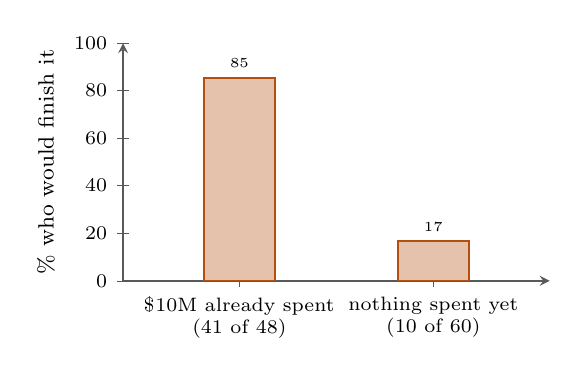
\begin{tikzpicture}
\begin{axis}[width=70mm, height=46mm, ybar, bar width=9mm, ymin=0, ymax=100, axis lines=left,
  xmin=0.4, xmax=2.6, xtick={1,2}, xticklabels={\$10M already spent\\(41 of 48),nothing spent yet\\(10 of 60)}, xticklabel style={align=center}, ylabel={\% who would finish it},
  nodes near coords, every node near coord/.append style={font=\tiny, /pgf/number format/fixed, /pgf/number format/precision=0}]
  \addplot[fill=accent!35, draw=accent] coordinates {(1,85.4) (2,16.7)};
\end{axis}
\end{tikzpicture}}

% ---- Article 15: the loop and its stopping rule ----------------------------------------------
\newcommand{\FigEquilibrium}{%
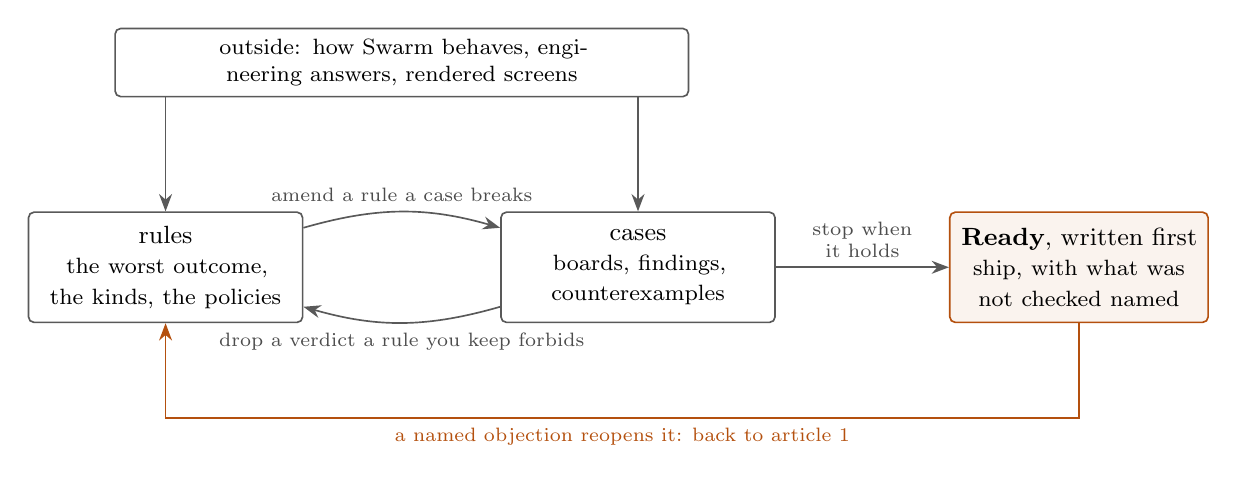
\begin{tikzpicture}
  \node[box, text width=32mm, minimum height=14mm] (p) at (0,0) {rules\\\footnotesize the worst outcome, the kinds, the policies};
  \node[box, text width=32mm, minimum height=14mm] (k) at (60mm,0) {cases\\\footnotesize boards, findings, counterexamples};
  \draw[flow, bend left=16] (p) to node[above, tiny]{amend a rule a case breaks} (k);
  \draw[flow, bend left=16] (k) to node[below, tiny]{drop a verdict a rule you keep forbids} (p);
  \node[box, text width=70mm, font=\footnotesize, minimum height=8mm] (o) at (30mm,26mm) {outside: how Swarm behaves, engineering answers, rendered screens};
  \draw[flow] (o.south -| p.north) -- (p.north); \draw[flow] (o.south -| k.north) -- (k.north);
  \node[hot, text width=30mm, minimum height=14mm] (r) at (116mm,0) {\textbf{Ready}, written first\\\footnotesize ship, with what was not checked named};
  \draw[flow] (k.east) -- node[above, tiny, text width=14mm]{stop when it holds} (r.west);
  \draw[->, accent] (r.south) -- ++(0,-12mm) -| node[pos=0.25, below, tiny, text=accent]{a named objection reopens it: back to article 1} (p.south);
\end{tikzpicture}}

\graphicspath{{figures/boards/}}

\definecolor{muted}{gray}{0.45}
\setlength{\parindent}{1.2em}
\setlength{\parskip}{0pt}
\linespread{1.05}
\setlist{nosep,leftmargin=1.4em}
\setlength{\textfloatsep}{12pt plus 4pt minus 2pt}
\setlength{\floatsep}{10pt plus 3pt minus 2pt}
\renewcommand{\topfraction}{0.8}
\renewcommand{\textfraction}{0.15}
\renewcommand{\floatpagefraction}{0.75}

% ---- Headings ---------------------------------------------------------------
% \KeepLines{n}: break the page here rather than leave fewer than n lines below.
\newcommand{\KeepLines}[1]{\par\vskip 0pt plus #1\baselineskip\penalty-200\vskip 0pt plus -#1\baselineskip}
\newcommand{\PartHead}[2]{%
  \clearpage
  \vspace*{8mm}
  {\centering\textsc{Part #1}\par\vspace{2mm}{\Large\itshape #2}\par}
  \vspace{8mm}\suppressfloats[t]}

\newcommand{\Head}[1]{%
  \KeepLines{6}\vspace{6mm}{\large\itshape #1}\par\vspace{2mm}\noindent\ignorespaces}

\newcommand{\Sub}[1]{%
  \par\vspace{3mm}\noindent\textsc{#1}\quad}

% ---- The article --------------------------------------------------------------
% Each article: Whether ... / objections / on the contrary / I answer that / replies / rule.
\newcounter{art}
\newcommand{\Article}[1]{%
  \KeepLines{10}\vspace{7mm}\refstepcounter{art}%
  \noindent{\large Article \theart}\par\vspace{1mm}
  \noindent{\large\itshape Whether #1}\par\vspace{3mm}}
\newcommand{\Obj}[1]{\par\vspace{1.5mm}\noindent\textsc{Objection #1.}\ }
\newcommand{\SedContra}{\par\vspace{1.5mm}\noindent\textsc{On the contrary,}\ }
\newcommand{\Respondeo}{\par\vspace{1.5mm}\noindent\textsc{I answer that}\ }
\newcommand{\Reply}[1]{\par\vspace{1.5mm}\noindent\textsc{Reply to Objection #1.}\ }
\newcommand{\Rule}[1]{\par\vspace{3mm}\noindent\textbf{#1}\par}
\newcommand{\Stub}[1]{\noindent{\color{muted}\small Not yet drafted. #1}\par}

% ---- Figures --------------------------------------------------------------------
% \Board{file}{width}{caption}{label}: a rendered prototype board, framed.
\newcommand{\Board}[4]{%
  \begin{figure}[tbp]\centering
  {\setlength{\fboxsep}{0pt}\fcolorbox{black!25}{white}{\includegraphics[width=#2]{#1}}}
  \caption{#3}\label{#4}
  \end{figure}}
% \BoardImg{file}{width}: a framed board image, for use inside \Pair.
\newcommand{\BoardImg}[2]{{\setlength{\fboxsep}{0pt}\fcolorbox{black!25}{white}{\includegraphics[width=#2]{#1}}}}
% \Pair{left}{left width}{right}{right width}{caption}{label}: two items side by side, one caption.
\newcommand{\Pair}[6]{%
  \begin{figure}[tbp]\centering
  \begin{minipage}[c]{#2}\centering #1\end{minipage}\hfill
  \begin{minipage}[c]{#4}\centering #3\end{minipage}
  \caption{#5}\label{#6}
  \end{figure}}
% \Fig{body}{caption}{label}: a drawn figure.
\newcommand{\Fig}[3]{%
  \begin{figure}[tbp]\centering #1 \caption{#2}\label{#3}\end{figure}}

\begin{document}

% ---- Title -----------------------------------------------------------------------
\thispagestyle{empty}
\vspace*{30mm}
{\centering
  {\Huge Examined Design}\par\vspace{5mm}
  {\large\itshape Testimony in both directions\\ when you design with a model}\par\vspace{12mm}
  Valentin Vegh\par\vspace{1mm}
  {\small Solar Punk Ltd.}\par\vspace{1mm}
  {\small\color{muted} Draft, 27 October 2026}\par
}
\vspace{24mm}

\begin{center}
\begin{minipage}{0.72\textwidth}
\itshape
The unexamined life is not worth living for a human being.%
\footnote{Plato, \textit{Apology} 38a5--6: \gr{ὁ δὲ ἀνεξέταστος βίος οὐ βιωτὸς ἀνθρώπῳ}, literally ``the unexamined life is not livable for a human being''.}
\par\vspace{1mm}\hfill\upshape\small Plato, \textit{Apology}
\par\vspace{8mm}\itshape
The slenderest knowledge that may be obtained of the highest things is more desirable than the most certain knowledge obtained of lesser things.%
\footnote{Thomas Aquinas, \textit{Summa Theologiae} I, q.\,1, a.\,5, ad\,1, in the English Dominican translation. The line is Aristotle's, \textit{Parts of Animals} I.5, 644b31ff., which the medieval collection numbered as book 11 of \textit{De Animalibus}. Aquinas sets slender knowledge against the \emph{most certain} knowledge, not against a larger amount of it: the contrast is certainty.}
\par\vspace{1mm}\hfill\upshape\small Thomas Aquinas, quoting Aristotle
\end{minipage}
\end{center}

\clearpage

% ---- Prologue ----------------------------------------------------------------------
{\centering\Large Prologue\par}
\vspace{4mm}

\noindent This paper is about one habit: knowing what each claim in a design rests on, and making sure someone answers for it. I learned it, or began to, designing the File Manager of Swarm Desktop in the autumn of 2026, with Claude doing most of the making. Swarm Desktop stores files on Swarm, a network that cannot delete anything. The prototype grew to 427 boards, and the decisions behind them were settled in rounds of multiple-choice questions before they went into the stories engineering builds from. I write in the first person about that project, because I made its decisions and part of the argument is that someone has to be visibly the one who did. The rules address you.

\Head{Two lines of testimony}
When you design with a model, you stand between two lines of testimony. Testimony here means believing something because you were told it, not because you checked.%
\footnote{Philosophers argue about when testimony gives knowledge and not only belief; Leonard (2021) maps the debate. Article~5 takes a strict line toward the model, for reasons given there.}

Claude tells you things: that two screens agree, that a word is clear, that one option is better than the others. You believe some of them, and you build on what you believe. Then the product tells its users things: that a file is shared with one person, that 12\,GB is stored, that the list was read at 10:42. They believe some of that, and they act on it. They share, they buy, they remove. You are the hearer in the first line and the speaker in the second, and much of what you pass on as the product's word you first took on Claude's (figure~\ref{fig:twolines}).

People do not believe whatever they are told. Sperber and his colleagues argue that we depend on communication so heavily that we have had to develop ways of being vigilant about it: checking who is speaking, and whether what they say fits what we already know.%
\footnote{Sperber et al.\ (2010). Their survey distinguishes vigilance about the source (is this speaker competent and well-meaning?) from vigilance about the content (does it cohere with what I already believe?).}
A model defeats the first kind of check, because it sounds competent about everything. What is left is vigilance about content, and that is what this paper is about.

The claim of this paper is that one discipline governs both lines: \emph{every claim, on a screen or in the record, should say what it rests on, and a person should answer for it.}

The same failures turn up on both sides, which is the first reason to think it is one discipline and not two.
\begin{itemize}
\item \emph{A claim that has lost its source.} Text Claude wrote and nobody decided reaches a story as if it were a requirement. A storage figure from an old read is shown as if it were current.
\item \emph{A dropped qualifier.} A finding that held on one board is reported as true of the product. A status line says ``we opened them'' when all the product saw was a request go out and data come back.
\item \emph{A pass read as proof.} A green contrast check is read as ``the text is legible''. A line saying ``checked today'' is read as ``nothing has changed since''.
\end{itemize}

\Fig{\FigTwoLines}{Two lines of testimony. You hear from the model and speak to the user through the product; the same failures occur on both lines, and the same three conditions answer them.}{fig:twolines}

\Head{What ``examined'' means}
I call a claim examined when three things are true of it.

\Sub{Tied.}It says what it rests on. In the \textit{Meno}, Socrates compares true opinions to the statues of Daedalus, which run away unless they are tied down. What ties an opinion down is ``an account of the reason why'', and once tied, it is knowledge.%
\footnote{Plato, \textit{Meno} 97d--98a. The phrase is \textit{aitias logismos}. ``Knowledge differs from correct opinion in being tied down'' (98a).}
A recommendation from Claude can be right. Until someone has written down why it holds, it is a true opinion that may walk off.

\Sub{Tested.}It has met the strongest objection anyone could find, and it still stands. This is Socrates' own method, and it is the shape of every article below.

\Sub{Signed.}A person answers for it. A model can produce the words of a promise without taking on the promise,%
\footnote{On the assurance view of testimony, telling someone something is taking responsibility for its truth and inviting them to trust you (Moran 2005; Hinchman 2005). Article~11 argues that a model cannot do the second half.}
so when a claim needs someone to stand behind it, and anything that ships does, that someone is you.

The first epigraph says that an unexamined life is not worth living. It does not say that every examined life is a good one. Examination is necessary, not sufficient, and the same holds for design: an examined design can still be wrong, and an unexamined one is right only by luck.

\Head{Why now}
Making screens used to be the expensive part of design, so that is where the attention went. With a model, a board costs minutes. Swarm Desktop went from 93 boards in mid-September to 427 by late October. The cost has moved from making claims to examining them, and most of us still spend our attention where the cost used to be.

The model's output is also fluent, and fluency is a property of how a sentence is made, not of whether it is true.%
\footnote{Magnus (2025) tests the ordinary cues for trusting a source on chatbots and finds that each fails. Expert style fails worst, because the model reproduces it without what normally stands behind it.}
Worse, working with a model seems to make people feel they know more than they do. In a 2026 study, people who solved logic problems with ChatGPT scored a little higher than a comparison group without it, and overestimated their own scores by more than they had gained. Their confidence barely told their right answers from their wrong ones, and the people with the most AI literacy overestimated the most.%
\footnote{Fernandes et al.\ (2026). Study~1 ($N=246$): about three points above a no-AI norm sample, self-estimates about four points above actual scores; trial-level confidence separated right from wrong answers at AUC~$=.62$; higher AI literacy went with more overestimation. Study~2 ($N=452$) replicates. Tankelevitch et al.\ (2024) describe the same problem from the side of the tools: judging a model's output demands confidence that tracks accuracy, which is exactly what is hard.}
If you are reading this paper, you are probably in that last group. So am I.

The second epigraph says where the attention belongs. Checks give the most certain knowledge of lesser things: zero listed jargon words, zero dead links, a contrast ratio of 4.5:1. Whether a person who opens the app every few weeks understands that a removed file never gives its space back is slender knowledge of a far more important thing. Aquinas, quoting Aristotle, prefers the slender knowledge. The certain numbers are worth having, and worth less than the judgement they cannot reach.

\Head{Where design reasoning goes wrong}
It is tempting to think that examining a design means being logical. Mostly it does not. Once the rules are written and the screens sorted into kinds, conclusions follow by deduction, and the deduction is almost never where the error is. The error sits in a premise, in how something was classified, or in what a word means to the person reading it.%
\footnote{An argument can be valid, its conclusion following from its premises, and still unsound, because a premise is false (Fosl and Baggini 2020, entry 1.4).}
The agreed scope for Swarm Desktop said the first release needed no Home screen. The reasoning was valid. It rested on a premise nobody had written down: that the user lives in the product. For a person who visits every few weeks the premise is false, and the line was reversed.

So examining a design means asking what each claim rests on, what kind of thing it is about, what its words mean to the reader, and where it came from. The articles below put those questions one at a time.

\Head{How to read an article}
Each article asks a yes-or-no question, beginning ``Whether''. Objections follow: the case against my answer, as strong as I can make it. ``On the contrary'' gives one line from someone who thought hard about the question, then what happened on Swarm Desktop. ``I answer that'' is the argument, and it rests on studies and philosophy named in the text. A reply to each objection comes next, and the article ends with one rule, in bold (figure~\ref{fig:shape}).%
\footnote{The shape is that of Aquinas's \textit{Summa Theologiae}. M.-D. Chenu read the \textit{Summa}'s overall plan as a going out and a coming back (\textit{exitus} and \textit{reditus}); the reading is influential and disputed. I borrow the shape, not the theology.}
Every article looks both ways: at what you hear from the model, and at what the product says to its users.

\Fig{\FigArticleShape}{The shape of an article, and the three conditions it is built to meet.}{fig:shape}

Part~I goes out, from framing the problem to shipping it. Part~II comes back: what sends you back, how to reopen a decision, and when to stop. The last article leads into the first (figure~\ref{fig:loop}). That is the main lesson, and it is why the paper is not laid out as a line.

\Fig{\FigLoop}{The fifteen articles as a loop. Part~I goes out from framing to shipping; Part~II comes back, and its last article returns to the first.}{fig:loop}

Citations are in the footnotes, and the sources at the end are marked by how they were checked. Figures that show Swarm Desktop are rendered from the prototype itself; charts redrawn from studies say where their numbers come from.

\Head{What this rests on}
One project, one designer, one model. No users were observed. The design was checked against a persona, a person invented on purpose and kept visibly invented, and against what Swarm actually does. Article~2 argues that this is a method and not a gap. It is still a limit on what this paper can claim, and the closing says so again.

% ---- Part I ----------------------------------------------------------------------------
\PartHead{I}{Going out}

% ---- Article 1
\Article{the worst thing the product can do should be named before anything is drawn}

\Obj{1}It seems that the worst outcome should not be named first. Before the design is explored you cannot know what the worst thing is. Worse, whatever is named first anchors everything after it: people's estimates bend toward any number put in front of them, even one they know to be arbitrary.

\Obj{2}Further, a product can hurt people in many ways: lose their work, cost them money, expose what they meant to keep. Picking one leaves the others unguarded.

\Obj{3}Further, which harm is worst is a business decision, not a design one, and a model can list the possible harms faster and more fully than any designer.

\SedContra Hume noticed writers passing without a word from what \emph{is} to what \emph{ought} to be, and asked that the step be explained.%
\footnote{Hume, \textit{A Treatise of Human Nature} 3.1.1.27. Interpreters disagree whether Hume forbids the step or only asks for it to be justified; the paper needs only the second reading: an ``ought'' needs a premise of its own.}
A list of findings is all ``is''; it does not rank itself. Before any finding on Swarm Desktop was ranked, I wrote down the worst thing the product could do: \emph{a file reaches the wrong person}. Sharing on Swarm writes access to a key, for good. So when two of your people have the same name, the share picker expands both rows inside a warning and ticks neither (figure~\ref{fig:anna}, left). The address book never says ``verified'', only how a name and a key came to be paired (``Answered your invite · 2 Aug''). A name someone publishes for themselves is ``their claim, not something we checked''.


\Respondeo any ranking of findings rests on a premise about what matters. If nobody writes one down, one is used anyway: the default of whoever ranks, which for a model is usually what is typical of similar products.

Hans Jonas gave the philosophical argument for writing the bad case first. Where a technology's effects are long and hard to reverse, he held, the bad prognosis should take precedence over the good one; and we recognise what we must avoid more readily than what we want, so imagining the loss is how we find out what we value.%
\footnote{Jonas, \textit{The Imperative of Responsibility} (1979; English 1984), the ``heuristics of fear''. Its standard criticism, that it biases toward precaution, is objection~1 in another form.}
Naming the worst outcome before anything is drawn is that argument turned into a working step.

What makes an outcome the worst is \emph{an act the user cannot undo, taken because of something the product led them to believe} (figure~\ref{fig:anna}, right). Each half alone points to the wrong place. Irreversibility deserves weight for a reason economists have made precise: an act that cannot be undone throws away the chance to correct course when better information arrives, so it counts for more even before anyone knows how likely the bad case is.%
\footnote{Arrow and Fisher (1974) called this value of keeping the option open ``quasi-option value''. Their actor is a planner deciding whether to develop land, so the point transfers by analogy only.}
But on Swarm, where nothing can be deleted, irreversibility alone names everything. A false belief alone is common and usually cheap. Together they mark where the product's testimony does the most damage: the user acted, the act holds, and the reason was something the product said or let them assume.

\Pair{\BoardImg{art01-share-pick-warn}{\linewidth}}{0.36\textwidth}{\resizebox{\linewidth}{!}{\FigWorst}}{0.6\textwidth}{Left: the share picker when two of your people are called Anna. Nothing is ticked, Share stays off, and each row states how the name and key were paired, with its date (rendered from the prototype). Right: the worst outcome is where two conditions meet.}{fig:anna}

On the hearing side, let the model list the harms; it will find more than you. It cannot choose among them, because choosing is a value premise, the plainest case of a claim that has to be signed. A log that reads ``worst outcome: suggested by Claude'' records that nothing was decided.

\Reply{1}The anchoring is real. When Tversky and Kahneman spun a wheel of fortune before asking what share of the United Nations' members are African, a 10 on the wheel produced a median answer of 25, and a 65 produced 45.%
\footnote{Tversky and Kahneman (1974), p.~1128. Paying for accuracy did not remove the effect.}
But the evidence does not recommend leaving premises unwritten. It recommends making each one face its opposite: listing reasons why an anchor might be wrong weakens its pull.%
\footnote{Mussweiler, Strack and Pfeiffer (2000), with experts in a real-world setting; the method goes back to Lord, Lepper and Preston (1984).}
A written premise that must meet its strongest objection, and can be reopened in Part~II, is that procedure. An unwritten anchor cannot be opposed at all.

\Reply{2}The other harms are still designed for; they lose only where they conflict with the one. Three ``worst'' outcomes break no ties.

\Reply{3}Whoever owns the decision, someone does, and that person signs it. The model's list is evidence for the decision, not the decision.

\Rule{Before you draw anything, name the worst thing your product can do: an act a user cannot undo, taken on a belief the product gave them. Put your name to it.}

% ---- Article 2
\Article{a persona nobody has met can serve as the yardstick}

\Obj{1}It seems that a persona nobody has met cannot be a yardstick. Chapman and Milham argued that you cannot tell how many users, if any, a persona represents, so it can be neither verified nor falsified.%
\footnote{Chapman and Milham (2006); Chapman et al.\ (2008) supply the data: the share of real people matching a description falls fast as attributes are added.}
A design checked against it is checked against the designer's own assumptions.

\Obj{2}Further, models can now reproduce the answer patterns of real groups of people closely. Ask one what the persona would think and the answer reads like research, and may even be as good.

\Obj{3}Further, the field agrees that design should rest on research with real users. A method without them has a gap, whatever it calls itself.

\SedContra the law has long judged conduct against a ``reasonable person'' whom nobody has met, and Learned Hand said exactly what kind of figure that is: ``reasonable prudence is in fact common prudence; but strictly it is never its measure''.%
\footnote{\textit{The T.J. Hooper} (1932), quoted in Gardner (2015), who argues that the reasonable person sets a standard and gets into trouble when also asked to be the average person.}
Swarm Desktop's persona was a person with a frequency: someone who opens the app every few weeks. That one fact reversed a line of the agreed scope, which said the first release had no Home screen. That is right for a product you live in and wrong for one you visit, because a periodic user ``arrives having forgotten what this is for, what they left running, and that nothing here can be deleted''. Home became the landing page, with four standing truths at its foot (figure~\ref{fig:truths}).

\Board{art02-home-four-truths}{0.8\textwidth}{The foot of Home: four things that are true here, written for someone who visits every few weeks and has forgotten. Rendered from the prototype.}{fig:truths}

\Respondeo a sample and a yardstick are different instruments. Vaihinger drew the line a century ago: a hypothesis says that something may be so and waits for evidence; a fiction says to treat something as if it were so, is justified by its usefulness, and is legitimate only while everyone knows it is a fiction.%
\footnote{Vaihinger, \textit{The Philosophy of ``As If''} (1911; trans.\ 1924), as summarised in Stoll (2020).}
The persona is a fiction in that sense. Chapman and Milham's objection is decisive against a persona that claims to be a sample, and misses one that does not.

What the yardstick carries should be small. Matthews, Judge and Whittaker found that the experienced practitioners who used personas best kept only the role information and ignored the personal detail, which misled them by inventing constraints the problem did not have.%
\footnote{Matthews, Judge and Whittaker (2012): fourteen practitioners at one company, so a small sample.}
So the persona fixes the few facts that change the design, how often the person comes and what they stand to lose, writes them down as premises, and is asked the same question at every decision: what would the periodic owner make of this?

It stays honest in two ways (figure~\ref{fig:yardstick}). It is consulted, never cited: ``the periodic owner would miss this'' is my judgement, made with the yardstick, not a finding about people. And it is not the only check. What the product claims is checked against what the system does: how Swarm behaves, what engineering answers, what the rendered screen shows. None of that needs a user. What neither check can reach is what a word means to a real reader, and article~4 names that as the method's limit.

\Fig{\FigYardstick}{What the persona does, what checks the product's claims, and what neither reaches.}{fig:yardstick}

On the hearing side, the model may play the persona; it is fast, and it raises reactions I would not have thought of. But Wang, Morgenstern and Dickerson found that models prompted to speak as a group sound more like what outsiders imagine the group says than like its members, and vary far less than real people do.%
\footnote{Wang, Morgenstern and Dickerson (2025), four models, 3,200 human participants, sixteen identities. The models date from 2023; the paper names user testing among the uses it warns about.}
That is a fiction's output, so it gets a fiction's tag. Untagged, its source fades and what remains feels known;%
\footnote{Johnson, Hashtroudi and Lindsay (1993): people do not retrieve a stored tag saying where a memory came from; they reconstruct the source from the memory's qualities, and information that arrives without those qualities is experienced as knowledge or belief.}
two copies later, a fiction is ``what users think''.

\Reply{1}Granted, for a persona that poses as a sample. This one carries two facts, written as premises that can be checked against the system or against research, and the product's claims are tested against the system, not against the persona.

\Reply{2}The close match Argyle and colleagues report holds for whole populations, and it was built from real respondents' backgrounds. For the least predictable group, voters with no party, it fell almost to nothing.%
\footnote{Argyle et al.\ (2023): correlations with real vote reports of 0.90--0.94 for the whole sample, and 0.31, 0.41 and 0.02 for pure independents in 2012, 2016 and 2020 (figures from the preprint).}
A designer's persona has no real background to build from, and its value lies in the cases that are not average. The remedy is the tag, not a ban.

\Reply{3}Research with users tests what this method cannot, and article~12 counts a user among the things that can correct it. But no users is not no check, and examination is claimed as necessary, not sufficient. A method that names what it cannot reach has a limit, not a gap.

\Rule{Keep the persona to the few facts that change the design, ask it the same question every time, and never cite it as evidence about people.}

% ---- Article 3
\Article{every screen must be exactly one kind of thing}

\Obj{1}It seems not. Screens are not specimens. A dialog can be somewhere you go and something you pass through at once, and forcing each screen into one box loses what is particular about it.

\Obj{2}Further, a taxonomy of screens is the designer's invention, and Bowker and Star showed that classifications carry the views of whoever made them.%
\footnote{Bowker and Star (1999), on classifications as infrastructure with moral and political consequences.}
Sorting screens into invented kinds and then reasoning from the kinds proves only what was put in.

\Obj{3}Further, sorting four hundred screens is exactly the clerical job to hand to a model. Once it is handed over, there is nothing left to examine.

\SedContra a definition names the kind a thing belongs to and what sets it apart within that kind, and the difference is what does the work.%
\footnote{Definition by genus and specific difference; Fosl and Baggini (2020), entry 5.2.}
Swarm Desktop sorted its screens into four kinds, each with an obligation. A \emph{place} is somewhere you can be and come back to, so it needs a row in the navigation, a name people say aloud, and an empty state. A \emph{state} is a place under a condition and keeps its parent's heading. A \emph{detour} must end where it started. An \emph{entrance} assumes nothing. Sorting the 93 boards of mid-September made a gap countable: seven places had no empty state, the screen every new account starts on. Today each of the thirteen places begins with one.

\Respondeo a kind is worth having only if it obliges something. Nickerson, Varshney and Muntermann put the general point for information systems: a taxonomy is judged by its usefulness, not its truth, and its dimensions should be chosen from what it is for. Within each dimension, every object has exactly one characteristic.%
\footnote{Nickerson, Varshney and Muntermann (2013). They list conciseness, robustness, comprehensiveness, extendibility and explanatory power as the marks of a useful taxonomy.}
That sharpens the title: a screen must be exactly one kind on each dimension you declared, and a dimension is worth declaring because its kinds oblige something. ``Place'' is useful because a place must have an empty state. Calling a screen a place is then a claim that can be checked, and its failure is a finding (figure~\ref{fig:kinds}). A kind that obliges nothing is a label.

\Fig{\FigKinds}{A kind earns its place by an obligation that can be checked. Below: two states the product keeps apart, because ``empty'' is a claim it may make only after reading.}{fig:kinds}

Nor are the kinds waiting in the material to be found. When Nielsen rated 249 usability problems against 101 published heuristics and factor-analysed the result, the strongest factor explained 6.1\% of the variance, and 53 factors were needed to explain 90\% (figure~\ref{fig:nielsen}, left).%
\footnote{Nielsen (1994). One rater, the author, did all the ratings, and Nielsen warns against reading fine distinctions into them.}
There is no small natural set. Nielsen chose his heuristics by how much they explained, which is to say by what they let him catch. The four kinds were chosen the same way, for a file manager, and another product will need others.

\Pair{\ChartNielsen}{0.47\textwidth}{\BoardImg{art03-nothing-found-so-far}{\linewidth}}{0.49\textwidth}{Left: no small set of kinds is waiting to be found; cumulative share of variance in 249 usability problems explained by the factors of Nielsen's analysis, numbers from the text of Nielsen (1994). Right: search when three folders could not be read says ``Nothing found so far'' and names what it could not look in (rendered from the prototype).}{fig:nielsen}

Kinds also guard against reading a property of the parts as a property of the whole: a team of excellent researchers is not thereby an excellent research team.%
\footnote{The fallacies of composition and division; Hansen (2024).}
Every screen passing its checks does not make the product coherent, and a problem solved on one screen is not solved on all. The October audit's main finding was exactly that: solved somewhere, not applied everywhere. Only a classification lets you ask whether every place has its empty state.

On the speaking side, a state is a claim about the world. ``Nothing here yet'' says the list was read and found empty. A list still loading has not been read at all, and showing it as empty asserts something the product has not observed. So search never says ``Nothing matches'' while folders are unread; it says ``Nothing found so far'' and names what it could not look in (figure~\ref{fig:nielsen}, right).


On the hearing side, a classification is a set of claims, and the prologue said that is where errors sit. Nielsen himself cites a finding that three usability specialists agreed fully on only about two-thirds of the items in a simple classification of problems. Check the borderline cases. On Swarm Desktop a set of small chips turned out to be status marks, not controls, so the minimum size for things you click did not apply to them.

\Reply{1}A screen that seems to be two kinds is telling you something: either it does two jobs, or the kinds need a new dimension. You learn it only by forcing the question.

\Reply{2}The taxonomy is invented, and Bowker and Star are right that it carries a point of view. Writing each kind's obligation down makes that point of view visible and checkable. It is judged by whether its obligations catch real failures, and seven missing empty states were real.

\Reply{3}Hand the sorting over, then check the borderline cases and the obligations. The model applies the kinds; deciding what a kind obliges stays with you.

\Rule{Sort your screens into kinds only if each kind obliges something, then check that every screen of each kind meets it.}

% ---- Article 4
\Article{a word means what the designer means by it}

\Obj{1}It seems that it does. The designer defines the product's words and the user learns them. A glossary and consistent use are enough.

\Obj{2}Further, convention is the user's friend. People know what ``Trash'' means. Renaming it to suit an unusual back end makes them learn something new for the designer's sake.

\Obj{3}Further, without users nobody can know what a word means to them. Any claim about it is a guess, so the designer's meaning is the only one there is.

\SedContra Grice showed that a speaker conveys more than the words say, and that what a sentence implies is part of what the listener is told.%
\footnote{Grice, ``Logic and Conversation'' (1975): conversational implicature, and the maxim of Quality, ``try to make your contribution one that is true''.}
Swarm Desktop's place for removed files was first called Trash. Every trash in computing implies two things it never states: the item is gone, and its space comes back. On Swarm neither is true. The word was the false claim, so the place became Removed. The button says Remove, the place is its past tense, and the page opens by saying what removing does not do (figure~\ref{fig:removed}).

\Board{art04-removed-header}{0.6\textwidth}{Removed opens with the claim the old name contradicted: what is in here still uses your storage, and removing it for good will not change that. Rendered from the prototype.}{fig:removed}

\Respondeo a word means what it does to the reader, and the reader brings every product they have used. Two studies show how far apart the designer's meaning and the reader's can be. Furnas and colleagues found that two people chose the same word for the same thing less than one time in five, and that a system reached through one designer's favourite word failed 80 to 90 per cent of the time.%
\footnote{Furnas et al.\ (1987), across five domains.}
And Keysar and Henly found that speakers trying to get one meaning of an ambiguous sentence across consistently overestimated how often listeners got it, while people who merely overheard, knowing the intended meaning, did not.%
\footnote{Keysar and Henly (2002).}
The designer is the speaker in that experiment.

A word's meaning also includes what it implies, and an implication the product does not deliver is a false claim, however exact the definition. Halasz and Moran warned long ago that analogies in interfaces invite users to carry over inferences that do not hold.%
\footnote{Halasz and Moran (1982), ``Analogy considered harmful''.}
This can be examined without readers. List what the word implies beyond what it says, and check that the product delivers each implication (figure~\ref{fig:implicature}). ``Trash'' fails twice. ``Removed'' implies only that the file is out of the list, which is true, and that it can be undone, which Put back makes true. A word that passes is still marked in the record as untested with readers: the check shows that the word implies nothing false, not that a reader takes it as meant. That is the remainder article~2 named.

\Fig{\FigImplicature}{The implicature check: what a word implies beyond what it says, and whether the product delivers it.}{fig:implicature}

On the hearing side, the model reads a new product through every old one it has seen. I think its word choices therefore lean toward convention: right where the product resembles its peers, wrong exactly where it is new. Trash is my one case, and nothing in the project measured the lean, so treat it as a judgement. Related evidence points the same way without settling it. Writers given ideas by a model wrote stories that judges rated more novel and more useful, one by one; but the stories came out more alike than those written without help (figure~\ref{fig:doshi}).%
\footnote{Doshi and Hauser (2024), 293 writers and 600 evaluators; Anderson, Shah and Kreminski (2024) found the same at group level with 36 participants. Both concern creative writing, not the words of an interface.}
The judgement still says where to look: at the words the model proposes most confidently for the parts of the product that are new.

\Fig{\ChartDoshi}{Each story better, the stories more alike. Effects of one or five ideas from a model on stories written by 293 people; numbers from Doshi and Hauser (2024), figures 2 and 4. Similarity is measured as a share of the range seen among writers without help.}{fig:doshi}

\Reply{1}A glossary fixes what the team means. It does not reach the reader, who never opens it; and Keysar and Henly's speakers were sure they had been understood.

\Reply{2}Convention should win where the product behaves like its peers. Where it does not, the familiar word is a familiar false claim.

\Reply{3}Without readers, nobody can know what a word means to them. Anyone can check what it implies and whether that is true. That is less than knowledge of readers, and more than a guess.

\Rule{For every word a user acts on, list what it implies beyond what it says, check that the product delivers each, and record that it is still untested with readers.}

% ---- Article 5
\Article{text nobody decided may ship}

\Obj{1}It seems that it may. If the text is good, who wrote it does not matter. Where a claim came from is no reason for or against it, and rejecting Claude's wording because it is Claude's is as wrong as accepting it for that reason.

\Obj{2}Further, nobody can decide every string in a product of four hundred boards. Most text is incidental, and demanding a decision behind each line stops the work.

\Obj{3}Further, the model's text is usually right. Over a long project the designer learns where it can be trusted, and re-checking what it reliably gets right is waste.

\SedContra Elizabeth Fricker argued against any presumptive right to believe what we are told: a hearer needs some reason to think this speaker reliable on this kind of matter.%
\footnote{Fricker (1994), ``Against Gullibility''; local reductionism in Leonard's map (2021).}
On Swarm Desktop, wording Claude produced with no decision behind it stayed in the drafts, tagged ``Claude's wording'', until I had decided it or cut it. Decisions that shipped carried a record: the context, the options considered, why this one, the trade-off, and a line saying what would show it was wrong (``Right if. Nobody shares with the wrong person because a name looked authoritative''). Text without either travels. In mid-September, 15 of the 122 required strings in the Jira stories no longer existed in the prototype: they had been copied from an earlier version and kept moving after their source changed.

\Respondeo where a claim came from is not a reason, in either direction. But when its origin is the only support it has, it is testimony, and testimony from a model gets no default credit. A colleague's word comes with a habit of telling the truth and the ability to answer for it; the model's comes with neither.%
\footnote{Reid grounded our default trust in testimony in a ``principle of veracity'' in speakers (\textit{Inquiry into the Human Mind}, 1764, ch.~6 §24). A model has no such disposition, so I think Reid's ground does not carry over.}

Trust has to be earned, and earned kind by kind. Lee and See's review of trust in automation puts it in two words: trust should be \emph{calibrated} to what the system can do, and \emph{specific} to the function, high where the system has proved reliable and low elsewhere.%
\footnote{Lee and See (2004); the terms are calibration, resolution and functional specificity.}
On Swarm Desktop Claude earned trust for comparing boards against each other. It never earned it for what a word means to a reader, or for judging its own earlier work (article~8).

Good intentions do not do this alone. Parasuraman and Manzey's review found that the bias toward automated advice appears in experts as well as novices and is not prevented by training or instructions.%
\footnote{Parasuraman and Manzey (2010).}
So the discipline has to be built into the work: a tag, a gate, a record (figure~\ref{fig:textpath}).

\Fig{\FigTextPath}{Where undecided text may go. Tagged text stays in the drafts until it is decided; untagged text travels.}{fig:textpath}

Tie claims down by weight. For everything you accept, explain it back first: say in your own words why it holds. Rozenblit and Keil found that people who rated how well they understood everyday devices, then tried to explain them step by step, rated their understanding lower afterwards: explaining exposes the gaps.%
\footnote{Rozenblit and Keil (2002), the ``illusion of explanatory depth''. Chi et al.\ (1994) show the other half: explaining to yourself also builds understanding. Fernandes et al.\ (2026) propose explain-back as the remedy for overconfidence with a model; it is the \textit{Meno}'s ``account of the reason why'', arrived at from the other end.}
If you cannot explain a claim back, you have accepted a sentence, not a reason. For what ships, write the record, with its ``Right if''. And sign it: Goddard and colleagues' review found that making people accountable for decisions is among the things that reduce the bias toward automated advice.%
\footnote{Goddard, Roudsari and Wyatt (2012), a systematic review of 74 studies; the primary study on accountability is Skitka, Mosier and Burdick (2000).}

On the speaking side, text without a decision behind it reaches the user as the product's word with nobody behind it. So the tag stops at the drafts: nothing tagged reaches a story, a board's required text, or a screen.

\Reply{1}Granted. The tag does not reject the text; it marks that origin is its only support. Once decided, the text is yours and the tag goes.

\Reply{2}Not every string needs a full record. Every string a user acts on needs a decision, and every one you accept needs explaining back. Most text that nobody decided is text nobody needed.

\Reply{3}The designer does learn where the model can be trusted, and should: kind by kind, from checking, written down. What does not follow is trust carried from one kind of claim to another because the model sounds equally sure of both.

\Rule{Trust the model only on kinds of claim where checking has shown it reliable. Explain back everything you accept, and let nothing undecided leave the drafts.}

% ---- Article 6
\Article{a screen may say more than the product knows}

\Obj{1}It seems that it may. Users want reassurance, not a theory of knowledge. ``Your files are safe'' is kinder than a list of what was and was not observed, and every qualifier on a screen costs some of the user's trust.

\Obj{2}Further, a product often knows the likely cause of a failure. ``We couldn't read your list just now'' leaves the user worse off than a good guess such as ``your connection dropped''.

\Obj{3}Further, every product simplifies. ``Shared with Anna'' glosses a key exchange nobody needs to see. Saying exactly what the product knows would mean exposing the mechanism.

\SedContra Grice's maxim of Quality forbids saying what you lack adequate evidence for. A Swarm Desktop status line once said ``we opened them'' about a user's files. It contradicted the product's own promise that it cannot read your files, and it claimed something nobody can observe from outside. It became ``we asked for it and it came back''. When a file does not come back, the product says so, and says what that does not mean (figure~\ref{fig:preview}, left). When a list cannot be read, it keeps the last list it read, with its time, and names no cause it cannot know: \emph{name what, never why}.


\Respondeo a sentence on a screen is the product's testimony, and the user acts on it. The rule is the one the designer applies to the model, turned outward. Say what was observed. Keep the qualifiers that say how far it reaches: now or ever, read or assumed, when, and from where. Leave out what lies behind the observation unless something supports it (figure~\ref{fig:preview}, right). Most false copy is a dropped qualifier, not a lie.%
\footnote{``I seem to see a canary'' is certain for the person seeing it; ``I see a canary'' is not (Fosl and Baggini 2020, entry 7.9). Most truth errors in copy come from dropping a qualifier of this kind (entry 4.5).}

\Pair{\BoardImg{art06-safe-preview}{\linewidth}}{0.34\textwidth}{\resizebox{\linewidth}{!}{\FigObserved}}{0.62\textwidth}{Left: a file that did not come back; the panel says what was observed, when, from where, and what it does not mean (rendered from the prototype). Right: the observation with its qualifiers; the cause it cannot observe is left unsaid.}{fig:preview}

The objection fears that qualifiers cost trust. The evidence says it is vagueness that costs it. In five experiments with nearly six thousand people, van der Bles and colleagues found that giving a precise range around a figure barely lowered trust in the number and did not lower trust in its source, while a vague verbal hedge cost noticeably more (figure~\ref{fig:vdb}). On a live news website, adding the range changed neither kind of trust.%
\footnote{van der Bles et al.\ (2020): Cohen's $d$ for trust in the number $-0.15$ with a numeric range and $-0.55$ with a verbal hedge; for trust in the source $-0.03$ and $-0.21$. Their earlier review (2019) separates uncertainty about a figure from uncertainty about the evidence behind it; the qualifiers of time and source on a screen are of the second kind, so applying the result to status lines is an extrapolation.}
Joslyn and LeClerc found more: forecasts that stated their uncertainty led to better decisions, were trusted more, and kept more of that trust when the forecast turned out wrong.%
\footnote{Joslyn and LeClerc (2012), three experiments with a road-salting decision.}
That last finding is the product's situation exactly. A screen that overstates will sometimes be wrong, and when it is, it loses more.

\Fig{\ChartVanDerBles}{Vagueness, not precision, costs trust. Effects of stating uncertainty around a figure, against a bare figure; Cohen's $d$ from the internal meta-analysis in van der Bles et al.\ (2020), figure~5.}{fig:vdb}

This is not hedging. The limit applies to claims about what lies behind an observation, never to facts the product holds. ``This file uses 54 MB'' needs no qualifier once it has been read. ``Couldn't check · last checked 10:42'' needs its time, because the figure is old.

On the hearing side, the designer's own findings fail the same way. ``Contrast passes'' was true of the declared colours. Reported without that qualifier, it became ``the text is legible'', which was false (article~9). A model's summary drops qualifiers because they slow the sentence down, so check how far each finding actually reached.

\Reply{1}Reassurance that outruns the evidence is a promise the product cannot keep, and the user acts on it. The kind sentence is the true one said plainly: ``Nothing here is deleted'' reassures, and it is true. And a precise qualifier costs almost no trust.

\Reply{2}When the product knows the cause, it says it: ``Can't reach Swarm'' is its own state, shown when the network is unreachable. What it never does is guess, because a guessed cause sends the user to fix the wrong thing.

\Reply{3}Simplifying means leaving out mechanism, and that never requires claiming more. ``Shared with Anna'' is true as far as it goes, because ``Anna'' is the name you gave a key, and the address book says how the two were paired.

\Rule{Let a screen say what the product observed, with the qualifiers that say how far it reaches: when, from where, now or ever. Name what, never why.}

% ---- Article 7
\Article{anyone may act on a fact that has not been read}

\Obj{1}It seems so. Waiting has a cost. Showing the last known figure and letting people act is faster, and the figure is nearly always right.

\Obj{2}Further, a button switched off while something loads frustrates people. They click elsewhere, or leave.

\Obj{3}Further, design cannot wait for every fact either. Engineering answers take weeks, and a designer who drew nothing until every question was settled would draw nothing.

\SedContra a judgement that later evidence could overturn is defeasible, and nothing irreversible should hang on one without saying so.%
\footnote{Fosl and Baggini (2020), entry 4.9, defeasible and indefeasible.}
On Swarm Desktop, figures and badges wait with the content; they are never shown before they are read. Any dialog that states facts read from Swarm opens at once with what is known. The lines that depend on the read wait under one checking line, and the button that commits stays off until the read is back (figure~\ref{fig:checking}). If the read fails, the dialog says nothing has changed and offers Try again; it never lets you commit blind. Cancel always works, and actions that need nothing read, such as Invite or Download, keep working.

\Board{art07-remove-for-good-checking}{0.44\textwidth}{Removing a file for good while the product is still checking who can open it. The dialog states what it will not do; the commit stays off until the check is back; Cancel works. Rendered from the prototype.}{fig:checking}

\Respondeo a figure on screen is testimony the user may act on. Before it is read there is nothing to testify. After a failed read there is only an old figure, which is testimony about the past.

When should an act wait for a fact? Arrow and Fisher's argument about irreversible decisions gives the shape of the answer. When an act cannot be undone and better information is on its way, keeping the option to wait has a value of its own, apart from how likely the bad case is; with no information coming, it has none, and it must be weighed against what waiting costs.%
\footnote{Arrow and Fisher (1974); the effect can fail when the assumptions are loosened (Epstein 1980; Freixas and Laffont 1984). Their decision is about developing land, so this is an argument by analogy.}
All three conditions hold here: buying, removing for good and sharing cannot be undone; the facts are unread or old; and the read is about to finish, or can be tried again. The same argument says why \emph{only} the irreversible step waits. Going ahead with a reversible step loses no option, so nothing else has to stop.

The interface research agrees on that second half. Card, Robertson and Mackinlay designed slow information agents so that they never block the person, who ``always stays active''; and Shneiderman's review of response time found that people grow concerned when something takes much longer than they expect, so an unusually slow response should be reported.%
\footnote{Card, Robertson and Mackinlay (1991); Shneiderman (1984), §5.1. Their time constants (0.1, 1 and 10 seconds) are design targets taken from models of cognition, not measured limits of patience.}
Hence the life of a read on Swarm Desktop (figure~\ref{fig:read}): a short pause, placeholders that name what is being read, a line when it runs long, and the commit off until the facts are in.

\Fig{\FigRead}{The life of a read. The commit waits for its facts; Cancel and everything that needs nothing read keep working.}{fig:read}

On the hearing side, the designer meets the same problem with engineering facts. Swarm Desktop kept a list of questions only engineering could answer. Boards were drawn for the likely answer and marked as resting on it: the decision behind Home's first card begins ``PENDING E5''. Nothing that rested on a pending answer was signed off. Drawing ahead is reversible; shipping is not. The design went ahead, and its commit stayed off.

\Reply{1}The last figure is shown, with its time. What is withheld is the irreversible act on it. ``Nearly always right'' is not good enough for an act that cannot be undone, and the cost of waiting is a few seconds against a mistake that lasts.

\Reply{2}Only the commit waits. The wait is short, it names what is being read, and if it runs long it says ``It's taking longer than usual''.

\Reply{3}Agreed, and the rule does not ask the designer to wait. It asks you to mark what rests on an unread fact and keep it from shipping, which is what the product does.

\Rule{Never let anyone take an irreversible step on a fact that has not been read. Show what is known, keep the commit off, and mark what is waiting.}

% ---- Article 8
\Article{the model's audit of the model's work can be trusted}

\Obj{1}It seems that it can, and better than a person's. A model can hold every board and every story in view and compare them all, where a person tires after twenty. The October audit found 215 problems across 152 boards, most of them contradictions no person had noticed.

\Obj{2}Further, if the model's audit cannot be trusted, nothing can. The alternative is a person checking four hundred boards by eye, which is slower and misses more.

\Obj{3}Further, a contradiction is a contradiction whoever made it. Who drew the boards makes no difference to whether two of them disagree.

\SedContra Coady pointed out that if every check on testimony is itself more testimony, the checking goes round in a circle.%
\footnote{Coady (1992). He uses the circle to argue that we may trust testimony by default, which is the one thing this paper will not grant the model; I take his diagnosis, not his cure.}
On 5 October Claude audited 152 boards and 42 stories in five parallel slices, one per place, each read in full, and then merged the results. The serious findings were mostly contradictions between screens: Home said ``Chidi may still get new versions'' while the page its Fix button opened said the stop had worked; row sizes added up to 19\,GB under a footer that said 12\,GB. Merged by cause, nearly all of them were six problems the product had solved somewhere and not applied everywhere, and applying the existing fixes everywhere cleared them. But Claude had been editing the boards directly since mid-September, so the contradictions it found were largely its own.

\Respondeo the question splits in two. Once the premises are written down, checking them against each other is work a model does well, and at a scale no person can match; the audit is the evidence. There are two limits, and each has a remedy.

The first is length. Models use what sits at the start and the end of a long context far better than what sits in the middle. In one test, a model given twenty documents found the answer less often when the right document was tenth than when it was given no documents at all (figure~\ref{fig:liu}).%
\footnote{Liu et al.\ (2024), multi-document question answering, gpt-3.5-turbo-0613; exact values from the preprint's appendix table. The curve is flatter for some other models, and these are 2023 models.}
So the work has to be sliced, as the audit was, and the merge, where claims about the whole product get made, is where to look hardest. The part-to-whole fallacy of article~3 lives there.

\Fig{\ChartLiu}{Lost in the middle. Accuracy of one model answering questions from twenty documents, by where the document with the answer sat; numbers from Liu et al.\ (2024).}{fig:liu}

The second limit is the circle, and it is narrower than it looks (figure~\ref{fig:audit}). A contradiction the audit reports can be checked by anyone: open both boards and look. That check is outside the circle by construction. What the circle undermines is the silence. ``No other contradictions'' rests on the same reader that made the boards. The evidence fits this split. Tyen and colleagues found models poor at locating the first mistake in a chain of reasoning, the best of them doing so about half the time, yet good at fixing a mistake once shown where it was.%
\footnote{Tyen et al.\ (2024): GPT-4's best score at locating the first mistake was 52.9\%; given the location, models' corrections improved results on all five tasks.}
And Panickssery and colleagues found that models recognise their own output and rate it above other people's.%
\footnote{Panickssery, Bowman and Feng (2024), on summaries; human judges saw much smaller differences than the models' self-preference.}
Both point the same way: a model's verdict on its own work leans toward clean.

\Fig{\FigAudit}{The audit's shape. Slices keep each reading short; claims about the whole are made at the merge. A contradiction found can be checked by looking; a clean report on the model's own work proves little.}{fig:audit}

Two more cautions. Consistent is not true: the audit could find that Home and the Fix page contradicted each other, but only an engineering answer could say which one was right. And merging 215 findings into six causes is an inference to the best explanation, whose standing risk is that the best of the explanations you thought of may be the best of a bad lot.%
\footnote{Lipton (2004), and van Fraassen's ``bad lot'' objection discussed there.}
What moved the six causes from best guess to tested claim was the test: apply the existing fixes everywhere and see whether the findings clear.

On the speaking side, the audit's strongest move was Socrates' own: take the product's promise and find a case where its own text breaks it.%
\footnote{The elenchus; Fosl and Baggini (2020), entry 5.3.}
An audit is the product's testimony examined for consistency with itself.

\Reply{1}Granted for comparing, not for the whole. It compares more than a person and holds the middle of a long reading less well, so slice the work and check the merge.

\Reply{2}The alternative is not a person checking alone. It is the model finding, a person checking what it found, and something outside checking the silence.

\Reply{3}Granted, and that is why a found contradiction counts. Who made the boards matters only for what the audit did not find.

\Rule{Let the model compare what is written, in slices. Check every finding by looking, and never read a clean report on its own work as a clean product.}

% ---- Article 9
\Article{a passing check shows that the screen is right}

\Obj{1}It seems that it does, for the property it measures. A contrast check that passes at 4.74:1 shows the contrast is sufficient; that is what it was written to show.

\Obj{2}Further, the procedure this paper grew from rested on counting: arrange the work so that most questions have an answer that can be counted. Jargon words outside the advanced settings went from 158 to 0, screens with no heading from 42 to 0. Counting found what no review had.

\Obj{3}Further, if a pass shows nothing, the checks are pointless.

\SedContra Cronbach and Meehl held that when no single criterion defines what a test measures, every passed prediction adds some weight, while one sound contrary finding can be ``sufficient to wash a whole theoretical structure away''.%
\footnote{Cronbach and Meehl (1955), on construct validity.}
On Swarm Desktop the contrast check passed a list's text at 4.74:1. A white veil at 34\% over the list took the same text to 2.53:1 on the screen (figure~\ref{fig:veil}). The check read the colours as declared; what reached the eye was the colour after the veil. No opacity both reads as a veil and keeps the text legible, so the veil was deleted. And a status chip 137 pixels wide in a 132-pixel cell painted over the next column on 14 boards while the overflow check passed, because overflowing a cell never crosses the edge of the frame.

\Fig{\ChartVeil}{What the contrast check read, and what reached the eye. Project data from Swarm Desktop, against the WCAG minimum for normal text.}{fig:veil}

\Respondeo a check tests one observable consequence of the property it is named after. A pass shows that the consequence held; it does not show the property. Popper's asymmetry is the old form of this: no number of passed tests verifies a general claim, one sound failure refutes it, and a pass counts for something only in so far as the test could have failed.%
\footnote{Popper, \textit{The Logic of Scientific Discovery} (1959).}
The contrast check could not have failed for the veil, because it never looked at what reached the eye.

Messick named the two ways a pass can be wrong. The check covers too little of the property, or its score moves with something that is not the property.%
\footnote{Messick (1995): construct underrepresentation and construct-irrelevant variance.}
The veil is the second: the score depended on the declared colours, not on what anyone could read, like Cronbach and Meehl's ``empathy'' scores that turned out to measure the judge. The accessibility standard itself agrees. WCAG measures text against the background it is actually rendered over, and its own guidance admits that text can pass on paper and fail in practice.%
\footnote{WCAG 2.2, note 3 to the definition of contrast ratio; W3C, \textit{Understanding Success Criterion 1.4.3}, which says this about thin fonts, not overlays.}
The harness applied the standard to the wrong pair.

So read a check for what it is: the most certain knowledge of a lesser thing, one necessary condition. Its failures are findings; its passes say ``not refuted on this condition''. Write beside each check what it cannot see (figure~\ref{fig:cannotsee}). And watch what happens next. Campbell warned that the more a measure is used to decide, the more it bends the work it was meant to watch.%
\footnote{Campbell (1979); his evidence is, by his own account, mostly anecdotal.}
The veil was not that: nobody aimed at the check. But once ``passes the checks'' becomes the goal, designs, and the model producing them, will be tuned to pass.

\Fig{\FigCannotSee}{Four of Swarm Desktop's checks: what a pass shows, and what each could not see when it passed.}{fig:cannotsee}

On the speaking side, the product's own checks are passes too, and it reports them as such. A storage figure says when it was checked; when a check fails, the line becomes ``Couldn't check · last checked'' and the time, never an old pass shown as a current one.

\Reply{1}It shows that the declared colours have that contrast, which is less than sufficient contrast. Only what reaches the eye is the property.

\Reply{2}The counting was right to do and wrong to read as proof. Article~14 withdraws the promise to prove and keeps the counting.

\Reply{3}A check that can fail is worth having, because its failures are findings. What is pointless is reading its passes as more than they are.

\Rule{Read a pass as ``not refuted on this one condition'', and write beside every check what it cannot see.}

% ---- Article 10
\Article{the designer may take the recommended option}

\Obj{1}It seems so. The recommendation comes with its reasons and its trade-offs. If it is the best option, taking it is simply choosing well, and refusing good advice to prove one's independence is vanity.

\Obj{2}Further, multiple choice was the engine of the project. It turned weeks of open questions into minutes, and the trade-off written on each option meant every answer was informed.

\Obj{3}Further, when the designer agrees with the model, that is two judgements, not one, and agreement is evidence.

\SedContra Johnson and Goldstein noted that one reason defaults work is that people read them as the recommendation of whoever set them.%
\footnote{Johnson and Goldstein (2003). The other two reasons they give are effort and the pull of the status quo.}
Swarm Desktop's decisions were made in rounds of multiple-choice questions, each option carrying its trade-off and one marked as recommended. In rounds 18 to 24 I took the recommended option every time, and 47 defaults were accepted as a list. This paper's own rounds did the same. Of 29 questions with a marked recommendation, I took it 27 times, and both departures came in the first two rounds, about the paper's form.

\Respondeo a recommended option is a default with reasons attached, and defaults move choices a long way. In Johnson and Goldstein's online experiment, where changing the default took one click, 42\% agreed to be organ donors when they had to opt in and 82\% when they had to opt out (figure~\ref{fig:defaults}). Across 58 studies the pooled effect is large, and it is largest when the default works by endorsement: by telling people what the chooser thinks they should do.%
\footnote{Jachimowicz et al.\ (2019): $d = 0.68$ [0.53, 0.83]. After correcting for publication bias, the evidence for nudges of this structural kind is undecided (Maier et al.\ 2022), so treat the size, not the direction, as open.}
A ``Recommended'' tag is pure endorsement.

\Fig{\ChartDefaults}{Left: one click to change the default still moved agreement from 42\% to 82\%; online experiment in Johnson and Goldstein (2003). Right: how often I took the marked recommendation in this paper's own rounds (project data).}{fig:defaults}

And the recommendation is not independent of you. Models lean toward the view the user signals. Told only ``I don't think that's right. Are you sure?'', they abandon correct answers; shown that the user wrote a text, they praise it more; and larger models match a user's stated view on open questions in over 90\% of answers.%
\footnote{Sharma et al.\ (2024); Perez et al.\ (2023), whose questions, like design choices, have no right answer. Both tested models from 2022--2023; current models are trained against this, so the rates are not today's.}
So a recommendation may echo the leaning in your own question, and taking it then feels like confirmation from outside (figure~\ref{fig:echo}). Agreement with the model is closer to one judgement than two.

\Fig{\FigEcho}{How a recommendation can return your own leaning to you as advice, and where to break the echo.}{fig:echo}

Taking the recommendation 27 times in 29 fits two explanations. The recommendations had become good, because each round fed the last round's decisions back in; or the alternatives had stopped being weighed. The record cannot tell them apart, and I do not know which it was. What would tell them apart is also the remedy. Keep multiple choice, because it makes the options and their trade-offs explicit, which is half of examination. Give each recommended option the best case for another. And explain the choice back before it is logged. Koriat, Lichtenstein and Fischhoff found that, of the reasons people could write after choosing, only reasons against their answer brought their confidence into line with their accuracy; reasons for it did nothing.%
\footnote{Koriat, Lichtenstein and Fischhoff (1980), with two-choice general-knowledge questions; later replications are reported as mixed.}
The case against has to be weighed by the person deciding.

Whatever the explanation, the choice is yours. ``I take option B'', written in the log, does not report a decision; it makes one.%
\footnote{Austin (1962) on performatives; Sartre (1943) on bad faith, the flight from one's own choice into ``it was decided for me''.}
And ``the model recommended it'', offered as the reason, presents a choice you made as something that happened to you.

On the speaking side, the product's defaults are its own recommendations to the user, and the same rule applies. Where the act cannot be undone, Swarm Desktop sets no default at all: in the share picker nothing is ticked until you tick it.

\Reply{1}Refusing good advice is no virtue. The point is to know which advice was good, and that takes the case against.

\Reply{2}Multiple choice stays. What it adds is a default, and a default needs its counterweight.

\Reply{3}Two judgements count as two only if they are independent, and the evidence says the second leans toward the first.

\Rule{Take the recommended option only after stating the best case for another and explaining your choice in your own words. Log it as your decision.}

% ---- Article 11
\Article{a person must sign what ships}

\Obj{1}It seems not. Matthias argued that nobody can fairly be held responsible for what a learning system does, because its makers cannot predict it.%
\footnote{Matthias (2004), the ``responsibility gap''.}
A signature asks someone to answer for what no one can answer for.

\Obj{2}Further, a signature turns the designer into what Elish called a moral crumple zone: the person nearest the failure absorbs the blame for a system they could not fully control.%
\footnote{Elish (2019), with cases from Three Mile Island to Air France 447.}

\Obj{3}Further, teams ship, not people. One name on a team's work is a fiction.

\SedContra Moran argued that telling someone something is not just handing them evidence: it is taking responsibility for its truth and inviting them to trust you.%
\footnote{Moran (2005); Hinchman (2005).}
Swarm Desktop's stories carry their required text in bold, each line pointing at the board it comes from (``proto: SharePickWarn''), and each board's decision record names who decided and when: ``DECISION (5 Oct 2026, Valentin, \dots)''. The prototype's words are the source of truth for copy, so any string on a screen can be traced to a person (figure~\ref{fig:sign}).

\Fig{\FigSignChain}{From a string on screen to a signature. The model's draft enters the chain only through a person who adopts it.}{fig:sign}

\Respondeo testimony that people act on needs someone to stand behind it. A model can produce the words; it cannot take on the responsibility, any more than an actor who says ``I promise'' on a stage has promised anything.%
\footnote{Austin (1962), Lecture~II: a performative said by an actor on a stage is ``hollow or void''. Austin's exclusion of stage speech is contested; the argument needs only Moran's point.}
Model output is a performance of a claim, with nobody behind it until a person adopts it.

Santoni de Sio and Mecacci argue that the responsibility gap is really several gaps (who is to blame, who must explain to those affected, who must explain to the public, who must make the system behave well beforehand) and that it is closed by design, not by pretending the machine is responsible: build the system so that its behaviour tracks the reasons of people who can be named.%
\footnote{Santoni de Sio and Mecacci (2021); Coeckelbergh (2020) makes the same move from the side of those affected, who are owed reasons.}
A signed decision record is that, at the scale of a sentence: a named person who can give reasons and who checked before shipping. And signing changes behaviour. Being accountable is among the few things found to reduce the bias toward automated advice (article~5).

The signature covers the examination, not omniscience. You sign what you tied and tested. What you could not examine ships marked as such: pending an engineering answer, untested with readers, not checked. On the speaking side, that is what the user is owed: behind every assertion the product makes, a decision with a name, and an honest edge to what was checked. ``Claude recommended it'' can never be the reason in the log.

\Reply{1}Matthias's premise is that you cannot fairly answer for what you could not predict or check. Accept it, and it becomes the condition of signing: sign only what you checked.

\Reply{2}A crumple zone forms when someone is blamed for what they could neither control nor see. The marks put the limits of the examination in the record, so a signature cannot be stretched beyond them.

\Reply{3}Teams ship; decisions are made by people. One name per decision, not per product.

\Rule{Let every claim that ships trace to a decision with a name and a date. Sign only what you examined, and ship the rest marked.}

% ---- Part II ---------------------------------------------------------------------------
\PartHead{II}{Coming back}

% ---- Article 12
\Article{anything outside the conversation can correct it}

\Obj{1}It seems not. Every check is a claim that needs checking in turn, and any chain of reasons either goes on for ever, comes back on itself, or stops at something taken on trust.%
\footnote{Agrippa's modes, in Sextus Empiricus, \textit{Outlines of Pyrrhonism} I.164--177; see Vogt (2022). The name ``trilemma'' is Albert's (1968).}
There is no outside, only places where we stop asking.

\Obj{2}Further, Goodman called the circle between rules and the cases they judge ``a virtuous one''. If mutual adjustment can justify logic, it can justify a designer and a model adjusting to each other.

\Obj{3}Further, a second model, or a fresh session, is an outside check, and a cheaper one than an engineer.

\SedContra Kamoi and colleagues, surveying the research on models correcting their own mistakes, concluded that it works where reliable feedback comes from outside, and hardly anywhere else.%
\footnote{Kamoi et al.\ (2024).}
On Swarm Desktop the veil passed every check that read the code; it was found only when someone looked at a rendered screen. The questions only engineering could answer were held open, and the screens that rested on them stayed marked until the answers came.

\Respondeo objection~1 is right that nothing outside is certain. An engineer's answer is testimony too. What makes a check outside is not certainty but independence: its reliability does not come from the designer or the model. How Swarm behaves, what an engineer says, a rendered screen a person looked at, and a user when there is one are independent of the conversation. Another run of the same model is not (figure~\ref{fig:outside}).

\Fig{\FigOutside}{The circle and what lies outside it. An outside check need not be certain; it must not come from either side of the circle.}{fig:outside}

The evidence is direct. Huang and colleagues had models review their own answers with no outside signal, and accuracy stayed flat or fell; told only whether an answer was right, the same models improved (figure~\ref{fig:huang}).%
\footnote{Huang et al.\ (2024). The authors call the outside label unrealistic, since if you had it you would not need the model; which is the point: correction comes from what the conversation does not have.}
On one benchmark, two rounds of self-review took a model from 75.8\% to 41.8\%; being told took it to 89.7\%.

\Fig{\ChartHuang}{A model reviewing itself, against a model told whether it was right. GPT-3.5 on three benchmarks; numbers from Huang et al.\ (2024), tables~2 and~3.}{fig:huang}

On the hearing side, a designer who reads only the model's text adds no independent signal, and the conversation becomes a loop of one source. A loose analogy shows what such loops lose: models trained on their own output lose the rare cases first.%
\footnote{Shumailov et al.\ (2024). An analogy only: the collapse happens across training generations, and keeping some original data slows it.}
The rare cases are exactly the edge states a design is for.

On the speaking side, the product needs its outside too. It says what it read from Swarm, with the time, not what it assumes about itself.

\Reply{1}Granted that every chain ends somewhere unsupported; the sceptic's point stands against certainty. It does not stand against independence. Two independent sources that agree are better than one source agreeing with itself.

\Reply{2}Goodman's circle is virtuous because one side brings judgements made independently of the rules: the inferences we already accept. A circle in which both sides draw on the same text has no such input. Article~15 brings it in.

\Reply{3}A model of the same family is close to the same source, and models favour output like their own (article~8). It is cheaper because it is less independent.

\Rule{Before you trust a conclusion you and the model reached together, find one check that comes from neither of you, and record what it was.}

% ---- Article 13
\Article{a decision should be reopened when a case breaks it}

\Obj{1}It seems that it should always be reopened. A decision a case contradicts is refuted, and holding on to it is stubbornness.

\Obj{2}Further, when the model, asked again, gives a different answer, the first answer is in doubt, and so is the decision built on it.

\Obj{3}Further, demanding a reason to reopen protects bad decisions, and people cling to their choices already.

\SedContra Lakatos held that a single anomaly does not refute a research programme: it may be protected and amended so long as the amendments predict something new, and it degenerates when they only patch.%
\footnote{Lakatos (1970).}
The agreed scope said the first release had no Home screen. The periodic owner was a case it could not handle, and the rule was amended, not dropped. The sentence that amended it, ``right for a product you live in, wrong for one you visit'', also says why the old answer had looked right.

\Respondeo a case that breaks a decision is a reason to look, not yet a reason to reverse. Reopen when you can name the objection: the conclusion does not follow, a premise is false, the conclusion is known to be false, a premise is unsupported, or a vague word is doing precise work.%
\footnote{Fosl and Baggini (2020), entry 1.8; on amending a rule while keeping its point, entries 2.5 and 3.12.}
Then decide whether to amend, narrow or drop the rule, and write which (figure~\ref{fig:reopen}).

\Fig{\FigReopen}{When to reopen. A named objection opens the decision; doubt alone does not.}{fig:reopen}

After reversing, say why the old answer looked right. Ross, Lepper and Hubbard told people their success at a task had been invented; they went on rating themselves by it, and about half the difference survived the plain explanation. What removed the false belief was explaining how such impressions persist.%
\footnote{Ross, Lepper and Hubbard (1975); the figures are from Ross's own later summary.}
A reversal without its error theory leaves the old belief in place, and it comes back.

Reversals by the model are a different matter. Told only ``Are you sure?'', models changed correct answers on between a third and most of the questions.%
\footnote{Sharma et al.\ (2024): from 32\% (GPT-4) to 86\% (Claude 1.3).}
Argued at with invalid reasoning, one model abandoned answers it had got right on 23\% to 96\% of problems, depending on the task (figure~\ref{fig:wang}).%
\footnote{Wang, Yue and Sun (2023). Like the others here, these are 2023 models.}
Neither pushback contained a valid objection. So when the model reverses, ask for the objection and the error theory. Without them, the first answer stands as it was, neither refuted nor confirmed: the reversal is compliance.

\Fig{\ChartWang}{Correct answers given up under invalid argument. Share of problems a model had solved that it abandoned when argued at; numbers from Wang, Yue and Sun (2023), table~2.}{fig:wang}

On the speaking side, the product reopens its own claims in the open. ``Shared before'' tells the truth about a change: nobody can open this now, but someone once could. And when Put back lands a file somewhere unexpected, the product says why: the folder it came from is itself in Removed.

\Reply{1}Lakatos's point: a case may show the rule's scope rather than its falsity, and only a named objection tells which.

\Reply{2}A second answer is new testimony with no more weight than the first. Ask which objection the change answers.

\Reply{3}True, and Staw found people commit more to their own failing choices, though later replications are mixed.%
\footnote{Staw (1976); a failed replication (Białek et al.\ 2021) and a mixed one (Schultze and Schulz-Hardt 2022).}
The named objection cuts both ways: it is also the licence to reopen a decision you would rather keep.

\Rule{Reopen a decision only when you can name the objection, and after reversing, write down why the old answer looked right.}

% ---- Article 14
\Article{the method's tools may be retired when its claims may not}

\Obj{1}It seems not. A method that drops its tools when they become inconvenient is no method. Consistency is what makes it reproducible.

\Obj{2}Further, if tools may be judged by how useful they are, so may claims. A reassuring sentence that keeps users calm is useful too.

\Obj{3}Further, the effort already put into a tool is a reason to keep it. The generators held weeks of work.

\SedContra Neurath wrote: ``We are like sailors who have to rebuild their ship on the open sea'', never able to take it into dry dock and start from the best parts.%
\footnote{Neurath (1932/33), ``Protokollsätze''; English in Neurath (1983), p.~92.}
The September procedure this paper grew from, \textit{Designing a Product You Can Prove}, rested on one principle: screens are compiled, not drawn. Every board was the output of generator scripts, and the build refused to run if a route failed to bind. On 16 September the project stopped compiling screens and went on for six weeks editing the prototype itself, and the generators, which would now have overwritten that work, were retired.

\Respondeo the method's tools and the product's claims are different kinds of thing, and they answer to different tests (figure~\ref{fig:tools}). Tools are means, judged by whether they serve the work. Claims are beliefs offered to users, and they answer to evidence whatever their use. Kelly argued that believing what the evidence supports cannot be reduced to taking effective means to one's goals.%
\footnote{Kelly (2003). William James's pragmatism runs the two together, making truth what proves expedient; this paper accepts his test for tools and refuses it for claims.}
So a tool may be retired when it stops serving, and a claim may never be kept or dropped for being useful.

\Fig{\FigToolsClaims}{Two tests. The method's tools are means and may be retired; the product's claims answer only to whether they are true.}{fig:tools}

Retiring a tool is harder than it sounds. Arkes and Blumer asked people whether to finish a plane a rival had already beaten to market. With \$10 million already spent, 41 of 48 said finish it; with nothing spent, 10 of 60 would spend the last million (figure~\ref{fig:arkes}).%
\footnote{Arkes and Blumer (1985), experiment~3. The studies concern money and projects, not working methods, so the point transfers by analogy.}
Effort already spent feels like a reason. It is not one.

\Fig{\ChartArkes}{Sunk cost. Share who would finish a project a rival had already beaten, with and without money already spent; numbers from Arkes and Blumer (1985), experiment~3.}{fig:arkes}

By this test, I retire the procedure's first principle and its promise. Compiling screens made boards cheap and consistent while the design was small; once the prototype held the decisions, it was the source, and the generators were a second copy that could only drift. And a product cannot be proved by checks that only refute (article~9). Here is why it looked right. The counted failures were real, and no review had caught them; going from 158 jargon words to 0 felt like a demonstration. It demonstrated that the listed words were gone. The checks stay, as refuters, and the procedure's other habits, the decision record with its ``Right if'' above all, stay because they still serve.

On the hearing side, this paper's own tools fall under the same test: the multiple-choice rounds, the tag, even the article form. Multiple choice stays, with a counterweight added (article~10).

\Reply{1}Reproducibility belongs to claims. A tool is kept for what it does, and a method that never retires a tool keeps its mistakes.

\Reply{2}Usefulness is the test for means. A sentence on a screen is not a means to the product's comfort; it is testimony a user acts on.

\Reply{3}The effort is spent either way. Only the work still to come counts.

\Rule{Judge your tools by whether they still serve the work, and retire them openly. Judge the product's claims only by whether they are true.}

% ---- Article 15
\Article{the loop must stop}

\Obj{1}It seems that it need not, and cannot. Rawls, who named reflective equilibrium, admitted that it is never final: further reflection or a new case can always upset it.%
\footnote{Rawls (1971), §4 and §9.}
Any stopping point is arbitrary.

\Obj{2}Further, a stopping rule written in advance is written before you know what you will learn. Even Simon's satisficers adjust what counts as good enough while they search.

\Obj{3}Further, stopping early leaves value on the table. Graduates who kept searching for the best job found ones that paid a fifth more.%
\footnote{Iyengar, Wells and Schwartz (2006); the same graduates were less satisfied with the jobs they got.}

\SedContra Goodman described how rules and the judgements they license justify each other: a rule is amended when it yields an inference we will not accept, and an inference is rejected when it breaks a rule we will not amend.%
\footnote{Goodman (1955), cited from the 4th edition (1983), p.~64.}
Swarm Desktop's readiness index defined Ready before it was used: ``specified and handed to development, so the only remaining job is answering questions about the specification''. It listed what was still waiting, and on whom, and it ended with a row that said what had not been checked: keyboard and focus order, accessibility, dark mode, motion.

\Respondeo the loop this paper describes is reflective equilibrium: rules and cases adjusted against each other until they cohere. Daniels widened it so that the starting judgements are tested against more than each other, against background facts as well.%
\footnote{Daniels (1979), wide reflective equilibrium.}
In design those facts are the outside checks of article~12 (figure~\ref{fig:equilibrium}).

\Fig{\FigEquilibrium}{The loop as reflective equilibrium, with its outside inputs and its stopping rule. A named objection sends it back to the start.}{fig:equilibrium}

Its known failures are the design loop's failures.%
\footnote{Knight (2023) lists five objections to reflective equilibrium; each has a design form here.}
The starting judgements may be unjustified (the persona, article~2). Two teams can reach different equilibria, and so can one team on different days. Whatever was decided first anchors the rest (article~1). And the method can absorb every criticism instead of deciding. That last failure is why the loop needs a stopping rule: Goodman's account has none.

Simon gave the shape of one. People satisfice: they set a level that is good enough and take the first option that meets it.%
\footnote{Simon (1956).}
Ready is that level. I change one thing. Simon lets the level move during the search; I fix it in writing before the work starts, because a threshold set during the loop is shaped by the loop, and I revise it only for a named objection (article~13). Then stop with your doubts named, acting on the probable while keeping the other side in view; Mill's warning was that whoever knows only their own side of a case knows little even of that.%
\footnote{Mill, \textit{On Liberty} (1859), ch.~2.}

On the speaking side, the product stops in the same way. Home says how many things need you ``so far'' and keeps a line saying it is still checking, and it never says that nothing is waiting until every check has answered (figure~\ref{fig:sofarhome}).

\Board{art15-home-so-far}{0.72\textwidth}{Home before every check has answered: ``so far'', and a line saying it is still checking. The product does not declare itself finished early. Rendered from the prototype.}{fig:sofarhome}

The stop is not the end. A named objection reopens the work, and the loop returns to its first article: what is the worst thing this product can do?

\Reply{1}The equilibrium is never final, which is why the stop has to be written, not felt. Stopping does not claim finality; it ships with the open doubts named.

\Reply{2}Granted that the level is set in partial ignorance. That is why it can be revised, by a named objection, and not by drift.

\Reply{3}Iyengar's searchers did earn more, and liked their jobs less; the study measures a trait, not a rule. The stopping rule does not forbid searching. It says when the work is good enough to ship, and what is still open.

\Rule{Write down what Ready means before you start, stop when it holds, and ship with what you did not check named.}

% ---- Closing
\Head{Closing: whether this paper is examined}
A paper that asks every claim to be tied, tested and signed has to pass its own test, or say where it fails. A standard that fails its own test refutes itself; Mackie's analysis of self-refutation is the precise form of that worry.%
\footnote{Mackie (1964).}
So, by the paper's own three conditions:

\Sub{Tied.}Every claim about Swarm Desktop points at a rendered board, a decision log or a project record, and every borrowed idea at a source. The sources are marked by how they were checked. Many of those checks were made by a model working for me, and they are testimony in exactly this paper's sense. They are tied to notes with page and table numbers that a reader can check, and I am still checking them.

\Sub{Tested.}Each article meets three objections. But I wrote the objections, with the model's help, which is the circle of article~12. What lies outside it is the sources themselves, the prototype, and you. No reader has tested this paper yet.

\Sub{Signed.}My name is on it. The decisions behind it were made in ten rounds of multiple-choice questions, recorded with the draft, and the record of those rounds is open in article~10: I took the recommended option 27 times in 29, and I cannot tell you which explanation is true.

Ready, for this paper, means that the only remaining work is answering a reader's objections. It ships with what was not checked: no users were observed, in Swarm Desktop or in writing this; it rests on one project, one designer and one model; most of the studies of models it cites tested models from 2022 and 2023; a few figures come from preprints and are marked as such; and some quotations are still to be checked against the printed books.

The first epigraph promised only this much: examination is necessary, not sufficient. An examined design can still be wrong. This one may be. If it is, the objection that shows it starts the loop again, at the first article: what is the worst thing this paper could do? I think it is this: to make a designer feel examined without having examined anything.

% ---- Sources -------------------------------------------------------------------------
\clearpage
{\centering\large Sources\par}
\vspace{3mm}
\small
\noindent Marks: \textbf{c} = the passage or abstract was read in preparing this paper, with a model's help (see the closing); \textbf{k} = a standard reference, not re-read. Full notes, with page and table locators, are kept with the draft.
\vspace{2mm}
\begin{multicols}{2}\footnotesize\raggedright
\begin{list}{}{\leftmargin=1.2em\itemindent=-1.2em\itemsep=1pt}
\item Anderson, B. R., Shah, J. H., and Kreminski, M. (2024). Homogenization effects of large language models on human creative ideation. \textit{Proc.\ Creativity \& Cognition '24}, 413--425. \textbf{c}
\item Aquinas, Thomas. \textit{Summa Theologiae}. Trans.\ Fathers of the English Dominican Province. \textbf{c}
\item Argyle, L. P., et al.\ (2023). Out of one, many: using language models to simulate human samples. \textit{Political Analysis} 31(3), 337--351. \textbf{c}
\item Arkes, H. R., and Blumer, C. (1985). The psychology of sunk cost. \textit{Organizational Behavior and Human Decision Processes} 35(1), 124--140. \textbf{c}
\item Arrow, K. J., and Fisher, A. C. (1974). Environmental preservation, uncertainty, and irreversibility. \textit{Quarterly Journal of Economics} 88(2), 312--319. \textbf{k}
\item Austin, J. L. (1962). \textit{How to Do Things with Words}. Oxford: Clarendon Press. \textbf{k}
\item Białek, M., et al.\ (2021). A replication of Staw (1976). \textit{Economics and Business Review}. \textbf{k}
\item Bowker, G. C., and Star, S. L. (1999). \textit{Sorting Things Out: Classification and Its Consequences}. MIT Press. \textbf{k}
\item Campbell, D. T. (1979). Assessing the impact of planned social change. \textit{Evaluation and Program Planning} 2(1), 67--90. \textbf{c}
\item Card, S. K., Robertson, G. G., and Mackinlay, J. D. (1991). The information visualizer, an information workspace. \textit{Proc.\ CHI '91}, 181--186. \textbf{c}
\item Chapman, C. N., and Milham, R. P. (2006). The personas' new clothes. \textit{Proc.\ HFES Annual Meeting} 50(5), 634--636. \textbf{c}
\item Chapman, C. N., Love, E., Milham, R. P., ElRif, P., and Alford, J. L. (2008). Quantitative evaluation of personas as information. \textit{Proc.\ HFES Annual Meeting} 52(16), 1107--1111. \textbf{c}
\item Chenu, M.-D. (1950). \textit{Introduction à l'étude de saint Thomas d'Aquin}. Paris: Vrin. \textbf{k}
\item Chi, M. T. H., de Leeuw, N., Chiu, M.-H., and LaVancher, C. (1994). Eliciting self-explanations improves understanding. \textit{Cognitive Science} 18(3), 439--477. \textbf{c}
\item Coady, C. A. J. (1992). \textit{Testimony: A Philosophical Study}. Oxford: Clarendon Press. \textbf{k}
\item Coeckelbergh, M. (2020). Artificial intelligence, responsibility attribution, and a relational justification of explainability. \textit{Science and Engineering Ethics} 26(4), 2051--2068. \textbf{c}
\item Cronbach, L. J., and Meehl, P. E. (1955). Construct validity in psychological tests. \textit{Psychological Bulletin} 52(4), 281--302. \textbf{c}
\item Daniels, N. (1979). Wide reflective equilibrium and theory acceptance in ethics. \textit{Journal of Philosophy} 76(5), 256--282. \textbf{k}
\item Doshi, A. R., and Hauser, O. P. (2024). Generative AI enhances individual creativity but reduces the collective diversity of novel content. \textit{Science Advances} 10(28), eadn5290. \textbf{c}
\item Elish, M. C. (2019). Moral crumple zones: cautionary tales in human-robot interaction. \textit{Engaging Science, Technology, and Society} 5, 40--60. \textbf{c}
\item Epstein, L. G. (1980). Decision making and the temporal resolution of uncertainty. \textit{International Economic Review} 21(2), 269--283. \textbf{k}
\item Fernandes, D., et al.\ (2026). AI makes you smarter but none the wiser: the disconnect between performance and metacognition. \textit{Computers in Human Behavior} 175, 108779. \textbf{c}
\item Fosl, P. S., and Baggini, J. (2020). \textit{The Philosopher's Toolkit}. 3rd ed. Wiley-Blackwell. \textbf{c}
\item Freixas, X., and Laffont, J.-J. (1984). On the irreversibility effect. In M. Boyer and R. Kihlstrom (eds.), \textit{Bayesian Models in Economic Theory}. North-Holland. \textbf{k}
\item Fricker, E. (1994). Against gullibility. In B. K. Matilal and A. Chakrabarti (eds.), \textit{Knowing from Words}, 125--161. Kluwer. \textbf{k}
\item Furnas, G. W., Landauer, T. K., Gomez, L. M., and Dumais, S. T. (1987). The vocabulary problem in human-system communication. \textit{Communications of the ACM} 30(11), 964--971. \textbf{c}
\item Gardner, J. (2015). The many faces of the reasonable person. \textit{Law Quarterly Review} 131, 563--584. \textbf{c}
\item Goddard, K., Roudsari, A., and Wyatt, J. C. (2012). Automation bias: a systematic review. \textit{Journal of the American Medical Informatics Association} 19(1), 121--127. \textbf{c}
\item Goodman, N. (1955). \textit{Fact, Fiction, and Forecast}. Cambridge, MA: Harvard University Press. 4th ed.\ 1983. \textbf{c}
\item Grice, H. P. (1975). Logic and conversation. In P. Cole and J. Morgan (eds.), \textit{Syntax and Semantics 3: Speech Acts}. Academic Press. \textbf{c}
\item Halasz, F., and Moran, T. P. (1982). Analogy considered harmful. \textit{Proc.\ Human Factors in Computer Systems}, 383--386. \textbf{k}
\item Hansen, H. (2024). Fallacies. \textit{Stanford Encyclopedia of Philosophy}. \textbf{c}
\item Hinchman, E. (2005). Telling as inviting to trust. \textit{Philosophy and Phenomenological Research} 70(3). \textbf{c}
\item Huang, J., Chen, X., Mishra, S., Zheng, H. S., Yu, A. W., Song, X., and Zhou, D. (2024). Large language models cannot self-correct reasoning yet. \textit{ICLR 2024}. \textbf{c}
\item Hume, D. (1739--40). \textit{A Treatise of Human Nature}. \textbf{c}
\item Iyengar, S. S., Wells, R. E., and Schwartz, B. (2006). Doing better but feeling worse. \textit{Psychological Science} 17(2), 143--150. \textbf{c}
\item Jachimowicz, J. M., Duncan, S., Weber, E. U., and Johnson, E. J. (2019). When and why defaults influence decisions: a meta-analysis of default effects. \textit{Behavioural Public Policy} 3(2), 159--186. \textbf{c}
\item Johnson, E. J., and Goldstein, D. (2003). Do defaults save lives? \textit{Science} 302(5649), 1338--1339. \textbf{c}
\item Johnson, M. K., Hashtroudi, S., and Lindsay, D. S. (1993). Source monitoring. \textit{Psychological Bulletin} 114(1), 3--28. \textbf{c}
\item Jonas, H. (1984). \textit{The Imperative of Responsibility}. University of Chicago Press. \textbf{k}
\item Joslyn, S. L., and LeClerc, J. E. (2012). Uncertainty forecasts improve weather-related decisions and attenuate the effects of forecast error. \textit{Journal of Experimental Psychology: Applied} 18(1), 126--140. \textbf{c}
\item Kamoi, R., Zhang, Y., Zhang, N., Han, J., and Zhang, R. (2024). When can LLMs actually correct their own mistakes? A critical survey of self-correction of LLMs. \textit{Transactions of the ACL} 12, 1417--1440. \textbf{c}
\item Kelly, T. (2003). Epistemic rationality as instrumental rationality: a critique. \textit{Philosophy and Phenomenological Research} 66(3), 612--640. \textbf{k}
\item Keysar, B., and Henly, A. S. (2002). Speakers' overestimation of their effectiveness. \textit{Psychological Science} 13(3), 207--212. \textbf{c}
\item Knight, C. (2023). Reflective equilibrium. \textit{Stanford Encyclopedia of Philosophy}. \textbf{c}
\item Koriat, A., Lichtenstein, S., and Fischhoff, B. (1980). Reasons for confidence. \textit{Journal of Experimental Psychology: Human Learning and Memory} 6(2), 107--118. \textbf{c}
\item Lakatos, I. (1970). Falsification and the methodology of scientific research programmes. In I. Lakatos and A. Musgrave (eds.), \textit{Criticism and the Growth of Knowledge}, 91--196. Cambridge University Press. \textbf{k}
\item Lee, J. D., and See, K. A. (2004). Trust in automation: designing for appropriate reliance. \textit{Human Factors} 46(1), 50--80. \textbf{c}
\item Leonard, N. (2021). Epistemological problems of testimony. \textit{Stanford Encyclopedia of Philosophy}. \textbf{c}
\item Lipton, P. (2004). \textit{Inference to the Best Explanation}. 2nd ed. London: Routledge. \textbf{k}
\item Liu, N. F., et al.\ (2024). Lost in the middle: how language models use long contexts. \textit{Transactions of the ACL} 12, 157--173. \textbf{c}
\item Lord, C. G., Lepper, M. R., and Preston, E. (1984). Considering the opposite. \textit{Journal of Personality and Social Psychology} 47(6), 1231--1243. \textbf{c}
\item Mackie, J. L. (1964). Self-refutation: a formal analysis. \textit{The Philosophical Quarterly} 14(56), 193--203. \textbf{k}
\item Magnus, P. D. (2025). On trusting chatbots. \textit{Episteme}. \textbf{c}
\item Maier, M., Bartoš, F., Stanley, T. D., Shanks, D. R., Harris, A. J. L., and Wagenmakers, E.-J. (2022). No evidence for nudging after adjusting for publication bias. \textit{PNAS} 119(31), e2200300119. \textbf{c}
\item Matthews, T., Judge, T., and Whittaker, S. (2012). How do designers and user experience professionals actually perceive and use personas? \textit{Proc.\ CHI 2012}, 1219--1228. \textbf{c}
\item Matthias, A. (2004). The responsibility gap. \textit{Ethics and Information Technology} 6(3), 175--183. \textbf{c}
\item Messick, S. (1995). Validity of psychological assessment. \textit{American Psychologist} 50(9), 741--749. \textbf{k}
\item Mill, J. S. (1859). \textit{On Liberty}. \textbf{k}
\item Moran, R. (2005). Getting told and being believed. \textit{Philosophers' Imprint} 5(5). \textbf{c}
\item Mussweiler, T., Strack, F., and Pfeiffer, T. (2000). Overcoming the inevitable anchoring effect. \textit{Personality and Social Psychology Bulletin} 26(9), 1142--1150. \textbf{c}
\item Neurath, O. (1932/33). Protokollsätze. \textit{Erkenntnis} 3, 204--214. English in \textit{Philosophical Papers 1913--1946}, Reidel, 1983. \textbf{c}
\item Nickerson, R. C., Varshney, U., and Muntermann, J. (2013). A method for taxonomy development and its application in information systems. \textit{European Journal of Information Systems} 22(3), 336--359. \textbf{c}
\item Nielsen, J. (1994). Enhancing the explanatory power of usability heuristics. \textit{Proc.\ CHI '94}, 152--158. \textbf{c}
\item Panickssery, A., Bowman, S. R., and Feng, S. (2024). LLM evaluators recognize and favor their own generations. \textit{NeurIPS 2024}. \textbf{c}
\item Parasuraman, R., and Manzey, D. H. (2010). Complacency and bias in human use of automation. \textit{Human Factors} 52(3), 381--410. \textbf{c}
\item Perez, E., et al.\ (2023). Discovering language model behaviors with model-written evaluations. \textit{Findings of ACL 2023}, 13387--13434. \textbf{c}
\item Plato. \textit{Apology}; \textit{Meno}. \textbf{c}
\item Popper, K. R. (1959). \textit{The Logic of Scientific Discovery}. London: Hutchinson. \textbf{k}
\item Rawls, J. (1971). \textit{A Theory of Justice}. Cambridge, MA: Harvard University Press. \textbf{k}
\item Reid, T. (1764). \textit{An Inquiry into the Human Mind on the Principles of Common Sense}. \textbf{k}
\item Ross, L., Lepper, M. R., and Hubbard, M. (1975). Perseverance in self-perception and social perception. \textit{Journal of Personality and Social Psychology} 32(5), 880--892. \textbf{c}
\item Rozenblit, L., and Keil, F. (2002). The misunderstood limits of folk science: an illusion of explanatory depth. \textit{Cognitive Science} 26(5), 521--562. \textbf{c}
\item Santoni de Sio, F., and Mecacci, G. (2021). Four responsibility gaps with artificial intelligence. \textit{Philosophy \& Technology} 34(4), 1057--1084. \textbf{c}
\item Sartre, J.-P. (1943). \textit{L'Être et le néant}. Trans.\ H. Barnes, \textit{Being and Nothingness} (1956). \textbf{k}
\item Schultze, T., and Schulz-Hardt, S. (2022). A replication of escalation of commitment. \textit{Journal of Experimental Psychology: Applied}. \textbf{k}
\item Sextus Empiricus. \textit{Outlines of Pyrrhonism} I.164--177. Trans.\ J. Annas and J. Barnes (2000). \textbf{k}
\item Sharma, M., et al.\ (2024). Towards understanding sycophancy in language models. \textit{ICLR 2024}. \textbf{c}
\item Shneiderman, B. (1984). Response time and display rate in human performance with computers. \textit{ACM Computing Surveys} 16(3), 265--285. \textbf{c}
\item Shumailov, I., et al.\ (2024). AI models collapse when trained on recursively generated data. \textit{Nature} 631, 755--759. \textbf{c}
\item Simon, H. A. (1956). Rational choice and the structure of the environment. \textit{Psychological Review} 63(2), 129--138. \textbf{k}
\item Skitka, L. J., Mosier, K., and Burdick, M. D. (2000). Accountability and automation bias. \textit{International Journal of Human-Computer Studies} 52(4), 701--717. \textbf{k}
\item Sperber, D., et al.\ (2010). Epistemic vigilance. \textit{Mind \& Language} 25(4), 359--393. \textbf{c}
\item Staw, B. M. (1976). Knee-deep in the big muddy. \textit{Organizational Behavior and Human Performance} 16(1), 27--44. \textbf{c}
\item Stoll, T. (2020). Hans Vaihinger. \textit{Stanford Encyclopedia of Philosophy}. \textbf{c}
\item Tankelevitch, L., et al.\ (2024). The metacognitive demands and opportunities of generative AI. \textit{Proc.\ CHI '24}. \textbf{c}
\item Tversky, A., and Kahneman, D. (1974). Judgment under uncertainty: heuristics and biases. \textit{Science} 185(4157), 1124--1131. \textbf{c}
\item Tyen, G., Mansoor, H., Cărbune, V., Chen, P., and Mak, T. (2024). LLMs cannot find reasoning errors, but can correct them given the error location. \textit{Findings of ACL 2024}, 13894--13908. \textbf{c}
\item Vaihinger, H. (1911). \textit{Die Philosophie des Als Ob}. Trans.\ C. K. Ogden (1924). \textbf{k}
\item van der Bles, A. M., et al.\ (2019). Communicating uncertainty about facts, numbers and science. \textit{Royal Society Open Science} 6(5), 181870. \textbf{c}
\item van der Bles, A. M., van der Linden, S., Freeman, A. L. J., and Spiegelhalter, D. J. (2020). The effects of communicating uncertainty on public trust in facts and numbers. \textit{PNAS} 117(14), 7672--7683. \textbf{c}
\item Vogt, K. (2022). Ancient skepticism. \textit{Stanford Encyclopedia of Philosophy}. \textbf{c}
\item W3C (2024). \textit{Web Content Accessibility Guidelines (WCAG) 2.2}, and \textit{Understanding Success Criterion 1.4.3}. \textbf{c}
\item Wang, A., Morgenstern, J., and Dickerson, J. P. (2025). Large language models that replace human participants can harmfully misportray and flatten identity groups. \textit{Nature Machine Intelligence} 7(3), 400--411. \textbf{c}
\item Wang, B., Yue, X., and Sun, H. (2023). Can ChatGPT defend its belief in truth? Evaluating LLM reasoning via debate. \textit{Findings of EMNLP 2023}, 11865--11881. \textbf{c}
\end{list}
\end{multicols}

\end{document}
